\documentclass[12pt,paper=a4]{report}
%%%% Maģistra/Bakalaura darba sagatave pēc VeA EPF nolikuma
%%$% Versija 0.1
%%%% Trūkst:
%%%% - Pēc nolikuma lapu numerācijai jābūt augšpusē?! - to var panākt ar fancy header
%%%% - Uzstādīt, lai \url rādītu arī kirilicu
%%%% - Kā iegūt visu zīmējumu, tabulu skaitu dokumentā
%%%% Vajadzētu papildināt ar:
%%%% - Tabulu un atsauču piemēri
%%%% - Formulu un atsauču piemēri
%%%% - Pielikumu lapu


%%%% Šeit izmantoti piemēri arī no Adriana Heidena un Arņa Voitkāna materiāli
%%%% Darbam ir jālieto xelatex ar latviešu valodas atbalstu  (Ubuntu sistēmās - jābūt texlive-lang-latvian un texlive-xetex)
%%%% Izveidoto tex failu (darbs.tex šai piemērā) 3x pēc kārtas (lai pareizi saliktos visas atsauces un satura rādītājis)
%%%% izveido ar komandu xelatex:
%%%% xelatex darbs.tex & xelatex darbs.tex & xelatex darbs.tex
%%%% Rezultātam jābūt failā darbs.pdf

% XeLaTeX atbalsts
\usepackage{fontspec}
\usepackage{xunicode}
\usepackage{xltxtra}
\usepackage{wrapfig}


\usepackage{rotating}
\usepackage{tikz}


% Valodu atbalsts
\usepackage{polyglossia}
\setdefaultlanguage{latvian}
\setotherlanguages{english,russian,french}

% Fonti -- var rakstīt sistēmas fontu nosaukumus
% Parastais teksta fonts
\setmainfont[Mapping=tex-text]{Times New Roman}%{LMRoman10}
% Fonts krievu valodai, kurā ir arī krievu valodas burti
\newfontfamily\russianfont{Times New Roman}
% Šos fontus tālāk izmantos chapter virsrakstos un url'os (lai būtu kirilicas burti)

\usepackage{setspace}

% lai varam normāli rakstīt apakšvītras
\usepackage{underscore}
% Lai varam iekļaut attēlus
\usepackage{graphicx}
% Kurā vietā tiks meklēti attēli - relatīvais ceļs attiecībā pret dokumentu
\graphicspath{{./PNG/}{./images/internet/}{./images/created/}}
% Ar šiem PDF'ā būs saliktas saites un tām va uzlikt krāsu
\usepackage{hyperref}
\hypersetup{ colorlinks, citecolor=black, filecolor=black,linkcolor=black,urlcolor=black }

\usepackage{amsmath}
\usepackage{amsfonts}
\usepackage{lipsum} %Lai ģenerētu nejaušus tekstus...
\usepackage{listingsutf8}
\usepackage{xcolor}

\usepackage{svg}
%\usepackage{inconsolata}
\lstset{
    language=bash, %% Troque para PHP, C, Java, etc... bash é o padrão
    basicstyle=\ttfamily\small,
    numberstyle=\footnotesize,
    numbers=left,
    backgroundcolor=\color{gray!10},
    frame=single,
    tabsize=2,
    rulecolor=\color{black!30},
    title=\lstname,
    escapeinside={\%*}{*)},
    breaklines=true,
    breakatwhitespace=true,
    framextopmargin=2pt,
    framexbottommargin=2pt,
    extendedchars=false,
    inputencoding=utf8
}

\usepackage{float}

%% Mainīt chapteru izskatu - centrēts un definētais sffamily fonts (skatīt augstāk)
\usepackage{titlesec}
\titleformat{\chapter}{\bfseries\LARGE\centering}{\thechapter}{1pc}{}
\titlespacing*{\chapter}{0pt}{-50pt}{40pt}
\newenvironment{conditions}
  {\par\vspace{\abovedisplayskip}\noindent\begin{tabular}{>{$}l<{$} @{${}={}$} l}}
  {\end{tabular}\par\vspace{\belowdisplayskip}}


%% Pārdēvējam ``Literatūra`` par ``Izmantotās literatūras un avotu saraksts''.
\addto\captionslatvian{
\renewcommand{\contentsname}{SATURS}%
\renewcommand\bibname{IZMANTOTĀS LITERATŪRAS UN AVOTU SARAKSTS}
}

%% Atraitņrindiņas un bāreņrindiņas ( widow orphan) vadība
\clubpenalty10000
\widowpenalty10000

%% Visādas atkāpes - 1" (2.54 cm) atkāpe jau ir pēc noklusējuma, šeit tikai korekcijas
%\setlength{\parskip}{1line}
\setlength{\topmargin}{0cm}
\setlength{\headheight}{0in}
\setlength{\headsep}{0in}
\setlength{\textheight}{22.7cm}
\setlength{\textwidth}{15cm}
\setlength{\oddsidemargin}{0.5in}
\setlength{\evensidemargin}{0.5in}
%\setlength{\parindent}{0.25in}
%\setlength{\parskip}{0.25in}

%% uzliekam atkāpes arī nodaļu 1. rindkopas 1. rindai
\usepackage{indentfirst}

%Pārnesumiem - ļauj tiasīt lielākas starpas
\hyphenpenalty=5000

%% Nodaļu un apakšnodaļu numerācija
\def\thechapter      {\arabic{chapter}.}
\def\thesection      {\ifx\chapter\undefined{\arabic{section}.}\else  {\thechapter\arabic{section}.}\fi}
\def\thesubsection   {\thesection\arabic{subsection}.}
\def\thesubsubsection{\thesubsection\arabic{subsubsection}.}
%\def\theparagraph    {\thesubsubsection\arabic{paragraph}.}
%\def\thesubparagraph {\theparagraph\arabic{subparagraph}.}

%% Pakotne lai saliktu automātisku figūru skaitīšanu
\usepackage{totcount}

\newcounter{nofappendices}
\setcounter{nofappendices}{0}
\regtotcounter{nofappendices}

\newcounter{formulanum}
\setcounter{formulanum}{0}
\regtotcounter{formulanum}

\newtotcounter{fignum}
\def\oldfigure{} \let\oldfigure=\figure
\def\figure{\stepcounter{fignum}\oldfigure}

%defineejam atsauču skaitītāju
\newtotcounter{citnum}
\def\oldbibitem{} \let\oldbibitem=\bibitem
\def\bibitem{\stepcounter{citnum}\oldbibitem}

%% Attēlu numerācija
\renewcommand{\thefigure}{\arabic{chapter}.\arabic{figure}.}
\renewcommand{\thetable}{\arabic{chapter}.\arabic{table}.}
\usepackage{tocloft}
%\renewcommand{\cftchapfont{\centering\sffamily}}
%\tocloftpagestyle{fancy}
\renewcommand{\cfttoctitlefont}{\hfill\Large\bfseries}
\renewcommand{\cftaftertoctitle}{\hfill\hfill}
\renewcommand{\cftpartleader}{\cftdotfill{\cftdotsep}} % for parts
\renewcommand{\cftchapleader}{\cftdotfill{\cftdotsep}} % for chapters
\renewcommand{\cftsecleader}{\cftdotfill{\cftdotsep}}

% %% Sarakstam visus mainīgos
% %% Mainīgie titullapai, defAutors tiek izmantots arī galvojumā

%% Sarakstam visus mainīgos
%% Mainīgie titullapai, defAutors tiek izmantots arī galvojumā
\def\defAutors{Gints Jasmonts}
\def\defAugstskola{Ventspils Augstskola}{\fontfamily{russianfont}}
\def\defFakultate{Informācijas tehnoloģiju fakultāte}
\def\defSProgrammas{bakalauru studiju programmas\\
	      datorzinātnēs}
\def\defStudents{3. kursa students \\
	      \defAutors}
\def\defMatrikulasNr{17020024}
\def\defDarbaNosaukums{Vāju radioastronomisko objektu novērojumu datu apstrāde - kalibrācija, filtrēšana un rezultātu analīze}
\def\defDarbaNosaukumsEN{Weak radioastronomical object observation data processing - calibration, filtration and result analysis}
\def\defDarbaNosaukumsLV{Vāju radioastronomisko objektu novērojumu datu apstrāde - kalibrācija, filtrēšana un rezultātu analīze}
\def\defDarbaVeids{Bakalaura darbs}
\def\defFakultatesDekans{Dr.~sc.~comp. Vairis Caune}
\def\defZinVaditajs{Mg.~sc.~comp. Karina Šķirmante}
\def\defGads{2020}
 %šeit pārdefinējam savus mainīgos (atstāju iepriekšējās rindas, lai varētu redzēt pārdefinēšanu)
\renewcommand\abstractname{ABSTRACT}
%% pievienota anotācijas noformēšana
%\usepackage{etoolbox}% http://ctan.org/pkg/etoolbox
%\makeatletter
%\patchcmd{\@makechapterhead}{\vspace*{50\p@}}{}{}{}% Removes space above \chapter head
%\setafterchapterskip{1sp}
%defineejam anotaacijas lapas, lai vareetu vienkaarshaak taas izmantot
\def\abstract{
  %\section*{\begin{center} \abstractname \end{center}} % start chapter

\vspace*{-4\baselineskip}
	\chapter*{\begin{center} \abstractname \end{center} } % start chapter
	\vspace*{-2.5\baselineskip}
  \addcontentsline{toc}{chapter}{\abstractname} % table of contents line
  \markboth{\MakeUppercase{\abstractname}}{} % header mark
}
\def\endabstract{}%\clearpage

%% Beidzot sākam rakstīt dokumentu
\begin{document}

%% Vislabāk nodaļas rakstīt kā atseviškus failus, kurus iekļauj ar input (.tex paplašinājums pats tiek pielikts klāt)
% \input{src/mag-titullapa} %% visu titullapu ērtāk ir turēt datnē mag-titullapa.tex, bet te mēs tomēr visu rakstīsim vienā vietā:

%%%% Titullapas sākums
%%%% Titullapas sākums
\begin{titlepage}
\begin{center}
\textsc{
\defAugstskola\\
\defFakultate}\\
\vspace{2em}
\textbf{\defDarbaVeids}\\
\vspace{2em}
{\LARGE \textbf{\defDarbaNosaukums}}\\
\vspace{2em}
\begin{tabular}{@{}r@{}l@{}}
\parbox[c]{0.4\textwidth}{Autors:}&
\parbox[t]{0.6\textwidth}{
\defAugstskola s\\
\defFakultate s\\
\defSProgrammas\\
\defStudents \\
Matrikulas~Nr. \defMatrikulasNr\vspace{0.7em}\\
\mbox{}\hrulefill\vspace{-0.4em}\\
{\scriptsize(paraksts)}\vspace{2em}} \\
\parbox[c]{0.4\textwidth}{Fakultātes dekāns:}&
\parbox[t]{0.6\textwidth}{
\defFakultatesDekans\vspace{.7em}\\
\mbox{}\hrulefill\vspace{-0.4em}\\
{\scriptsize(paraksts)}\vspace{2em}} \\
\parbox[c]{0.4\textwidth}{Zinātniskais vadītājs:}&
\parbox[t]{0.6\textwidth}{
\defZinVaditajs\vspace{.7em}\\
\mbox{}\hrulefill\vspace{-0.4em}\\
{\scriptsize(paraksts)}\vspace{2em}} \\
\parbox[c]{0.4\textwidth}{Recenzents:} & \vspace{.7em}\\
\multicolumn{2}{@{}c@{}}{
\mbox{}\hrulefill
}\vspace{-0.4em}\\
\multicolumn{2}{@{}l@{}}{
{\scriptsize(Ieņemamais amats, zinātn. nosaukums,
vārds, uzvārds)}
}\vspace{.7em}\\
&\mbox{}\hrulefill\vspace{-0.4em}\\
&{\scriptsize(paraksts)}\\
\end{tabular}
\vfill
Ventspils, \defGads
\end{center}
\end{titlepage}
 %pievienota titullapa, kura izveidota atsevišķā failā
%%%% Titullapas beigas

%%%% Satura rādītājs

\tableofcontents

% Removes the page counter
\addtocontents{toc}{
\protect\thispagestyle{empty}} 
\thispagestyle{empty} 
\newpage

%%%% 1.5 līiniju atstarpe starp rindām
\onehalfspace

%%%% Nodaļa bez numerācijas
\chapter*{ANOTĀCIJA}
%%%% Lai uzrādītos satura rādītājā
\addcontentsline{toc}{chapter}{ANOTĀCIJA}
\begin{tabular}{@{}r@{}l@{}}
\parbox[c]{0.3\textwidth}{\textbf{Darba nosaukums:}}&
\parbox[t]{0.65\textwidth}{\defDarbaNosaukums} \\
\parbox[c]{0.3\textwidth}{\textbf{Darba autors:}}&
\parbox[t]{0.65\textwidth}{\defAutors} \\
\parbox[c]{0.3\textwidth}{\textbf{Darba vadītāja:}}&
\parbox[t]{0.65\textwidth}{\defZinVaditajs} \\
\parbox[c]{0.3\textwidth}{\textbf{Darba apjoms:}}&
\parbox[t]{0.65\textwidth}{\textcolor{black}{54} lapas, 3~tabulas,  \total{fignum}~attēli, 17~formulas, \total{citnum}~literatūras avoti, \total{nofappendices}~pielikumi} \\
\parbox[c]{0.3\textwidth}{\textbf{Atslēgas vārdi:}}&
\parbox[t]{0.65\textwidth}{ OH MĀZERI, KOMĒTAS, VĀJI SIGNĀLI, DATU APSTRĀDE, AUGSTAS VEIKTSPĒJAS SKAITĻOŠANA, ALGORITMI PARALĒLĀ REŽĪMĀ } \\
&\\

\end{tabular}
%\total{nofimages} % ja nu gadiijumaa vajag custom counter

Bakalaura darba mērķis ir veikt vāju radioastronomisko objektu datu apstrādi, to kalibrāciju,  trokšņa filtrēšanu, analizēt un apkopot iegūtos rezultātus. Primāri tiek novēroti OH māzeri Saules sistēmas komētu iekšienē, kuri, tuvojoties Saulei, aktivizējas un uzsāk OH molekulu izstarošanu. Balstoties uz to, ka komētas daļēji sastāv no ledus maisījumiem, novērojumi var sniegt informāciju par ūdeni kosmosā, kā arī ūdens rašanos uz Zemes. Darbā tiek arī novēroti un apstrādāti daži ārpus Saules sistēmas objekti, kā maiņzvaigznes un zvaigžņu veidošanās reģionu OH māzeri.  Lai to realizētu, izmantots RT-32 teleskops, ar kuru tiek veikti novērojumi diapazonā, kurā atrodas OH molekulu spektrālās līnijas - 1665MHz un 1667MHz.  Ņemot vērā, ka Ventspils Starptautiskais Radioastronomijas Centrā ar komētu novērojumiem darbs uzsākts tikai nesen, ir nepieciešams izveidot metodiku, kā plānot un apstrādāt iegūtos datus no minēto klasifikāciju radioastronomiskajiem avotiem. 

Bakalaura darba praktiskajā daļā Python valodā tika izveidoti datu apstrādes metodikā iekļautie algoritmi (kalibrācijas, trokšņa mazināšanas un spektra iegūšanas, apvienojot vairāku novērojumu rezultātus), kas veic darbības paralēli, izmantojot Message Passing Interface protokolu, tādējādi efektīvāk pielietojot VSRC augstas veiktspējas skaitļošanas nodaļai pieejamos skaitļošanas resursus. Darbā algoritmi tiek aprakstīti un izvērtēti, kā arī tiek aprakstīti potenciālie uzlabojumi, ko iespējams veikt. Darbā tiek apskatīti arī potenciālie uzlabojumi un nākotnes plāni datu apstrādes metodikā.


Darba rezultātā ir iegūta metodika, uz kuras balstoties, ir iespējams apstrādāt vāju starojuma astronomisko objektu radio astronomiskos datus. Bakalaura darba apraksta ietvaros tiek apskatīts metodikas pielietojums uz ATLAS Y4/2019 komētas, kā arī tiek apskatīti rezultāti maiņzvaigznei R Leonis Minoris un citiem novērotajiem objektiem.






%Anotācija (lat. \textit{annotatio} – piezīme) ietver īsas ziņas par maģistra un bakalaura darba mērķi un risināmiem uzdevumiem, saturu, pielietotajām metodēm, galvenajiem izmantotajiem informācijas avotiem, pētījuma problēmām un svarīgākajiem rezultātiem, tabulu, attēlu skaitu u.c. ziņas. Anotācijā arī jānorāda, kādu zinātnisku vai praktisku jautājumu risināšanā darbs varētu būt izmantojams.

%Šis ir paraugs, kurā ir izmantoti Adriana Heidena\footnote{A.Heidens bija VeA students} un Arņa Voitkāna materiāli\footnote{\url{http://blogi.lu.lv/arnivoit/latex-un-docbook-instalesana/latex-latviesu-valodas-atbalsta-konfiguresana-uz-linux-un-windows/}}

%Ja pēdējā lapā ierakstīsim \verb+\label{LastPage}+, tad šeit anotācijā rakstot ar \verb+\pageref{LastPage}+ tiks ierakstīts kopējais lapu skaits. Ar kopējo zīmējumu un tabulu skaitu ir sarežģītāk, tos numurē nodaļas ietvaros un tāpēc ir jāizveido jauns skaitītājs - tas gan te netiek aprakstīts.

%Bakalaura darbā ir \pageref{LastPage}  lapas, un \total{fignum} attēli.


%{
%% selectlanguage nav obligāti, ja raksta tikai tekstu un standarta fontā ir kirilicas simboli.
%\selectlanguage{russian}
%\chapter*{Аннотация}
%\addcontentsline{toc}{chapter}{Аннотация}
%В книге Дугласа Адамса «Путеводитель для путешествующих автостопом по галактике» «Ответ на главный вопрос жизни, вселенной и всего такого» должен был решить все проблемы Вселенной. Этого ответа с нетерпением ждали все разумные расы. Он был получен в результате семи с половиной миллионов лет  непрерывных вычислений на специально созданном компьютере Deep Thought. По утверждению компьютера, ответ был несколько раз проверен на правильность, но он может всех огорчить. Оказалось, что ответ на вопрос — «42». В ответ на недоумение представителей разумных рас, компьютер обосновал свой ответ тем, что формулировка вопроса была также весьма спорной.
%% Anotācijās nav citātu, bet mēs tos pieliksim, deomnstrācijas pēc
%% ievērojiet, ka te nav jaunas rindiņas sākums, jo nav tukšas rindas pa vidu
%% pašu citāta atsauci jāieraksta arī beigās - \thebibliography sadaļā
%\cite{wiki-ru}

%Настоящая магистерская работа содержит \pageref{LastPage} страниц и \total{fignum} рисунков.
%}

%%%% 1.5 līiniju atstarpe starp rindām
\onehalfspace
{
\selectlanguage{english}
\chapter*{ABSTRACT}
%%%% Lai uzrādītos satura rādītājā
\addcontentsline{toc}{chapter}{ABSTRACT}

\begin{tabular}{@{}r@{}l@{}}
\parbox[c]{0.3\textwidth}{\textbf{Title:}}&
\parbox[t]{0.65\textwidth}{\defDarbaNosaukumsEN} \\
\parbox[c]{0.3\textwidth}{\textbf{Author:}}&
\parbox[t]{0.65\textwidth}{\defAutors} \\
\parbox[c]{0.3\textwidth}{\textbf{Academic Advisor:}}&
\parbox[t]{0.65\textwidth}{\defZinVaditajs} \\
\parbox[c]{0.3\textwidth}{\textbf{Volume of the work:}}&
\parbox[t]{0.65\textwidth}{\textcolor{black}{54} pages, 3~tables,  \total{fignum}~images, 17~equations, \total{citnum}~literature sources, \total{nofappendices}~appendices} \\
\parbox[c]{0.3\textwidth}{\textbf{Keywords:}}&
\parbox[t]{0.65\textwidth}{ OH MASERS, COMETS, WEAK SIGNALS, DATA PROCESSING, HIGH PERFORMANCE COMPUTING, PARALLEL ALGORITHMS} \\
&\\
\end{tabular}



The goal of this Bachelors degree thesis is to perform weak radioastronomic object data processing, which entails calibration, noise filtering and the analysis of results.  Primarily, OH masers from within comets in Solar system are observed, which upon getting closer to Sun activate and start emitting OH molecules, but observations on objects outside Solar system, such as stars and OH masers from star forming regions, are also performed. Considering that comets are mostly made of ice, observations may give us more insight about water in space, which includes the appearance of water on Earth. To perform the task, RT-32 radio telescope is used to observe the radio wave region of which spectral lines of OH molecules may be observed.  Since Ventspils International Radio Astronomy Centre has not performed comet observations until recently, there was no guidelines for data processing of such objects.  

There are a number of algorithms for radio telescope data processing created during the writing period of this thesis. Algorithms are written using the Python programming language and are crucial for observation data transformation, calibration, signal noise reduction and data aggregation, some of which are parallelized using the Message Passing Interface to efficiently use the high performance computing resources of VIRAC. Algorithms are explained and the potential improvements are noted. Potential improvements on the guidelines of OH maser observation data processing are also looked at.

%To use the high performance computing resources of VIRAC, an algorithm using MPI protocol is used for data processing is created along side with other data processing algorithms for signal noise reduction and result aggregation. Algorithms are explained and the potential improvements are noted.

As a result of this thesis, a set of instructions for successful OH maser observation data processing is produced and examples from a couple of observed objects, such as comet ATLAS Y4/2019 and Mira varible star R Leonis Minoris are examined.
%\total{nofimages} % ja nu gadiijumaa vajag custom counter

%In the first novel and radio series, a group of hyper-intelligent pan-dimensional beings demand to learn the \textbf{Answer to the Ultimate Question of Life} from the supercomputer, Deep Thought, specially built for this purpose. It takes Deep Thought 7½ million years to compute and check the answer, which turns out to be\textbf{ 42}.  Unfortunately, The Ultimate Question itself is unknown.\cite{wiki-en}


}



%%%% Nodaļa bez numerācijas
\chapter*{IZMANTOTIE SAĪSINĀJUMI UN TERMINI}
\addcontentsline{toc}{chapter}{IZMANTOTIE SAĪSINĀJUMI UN TERMINI}

%\textbf{Pievienot visus saīsinājumus un terminus, vairāk paskaidrot minētos}


\textbf{MPI} - Message Passing Interface protokols, Bakalaura darba ietvaros tiek izmantots, lai veiktu komunikāciju starp vairākiem \textit{Python} procesiem gan vienas iekārtas, gan vairāku skaitļošanas mezglu ietvaros.

\textbf{Novērojums} - Teleskopa fiziski pozicionēšana pret objektu uz noteiktu laiku un datu ierakstīšana laika periodā (parasti 2-4 stundas).

\textbf{Skans} - Novērojuma fragments, kurā ietilpst visas fāzes aptuveni 2 minūšu novērojuma intervālā. 

\textbf{FFT} - Fast Fourier Transform. Algoritms, kurš aprēķina diskrēto Furjē transformāciju, kura pārveido signālu frekvenču reprezentācijas modelī.

\textbf{Ns} - Furjē transformācijas rezultējošais garums

\textbf{VSRC} - Ventspils Starptautiskais Radioastronomijas Centrs

\textbf{VIRAC} - Ventspils International Radio Astronomy Centre

\textbf{Māzeris} - (Angliski \textit{maser}). Microwave Amplification by Stimulated Emission of Radiation. Dažu mikroviļņu starojuma pastiprināšanās sakarā ar inducētā starojuma rašanos komētas molekulās.

%\textbf{Vājš objekts} - Objekts, precīzāk tā OH māzeris, kurš izstaro vāju radiosignālu

\textbf{CSV} - Comma Separated Value. Faila formāts, kur vērtības atdalītas ar atdalīšanas simbolu, bieži - komatu.

\textbf{Dat formāts} - Formāts, kur kolonnās ierakstītas radioastronomiskā novērojuma rezultātā iegūtās vērtības. 

\textbf{Jēldati} - Binārais datu formāts, kur spektrs ierakstīts reālu un imagināru skaitļu virknē.

%\textbf{Doplera efekts} - Frekvences izmaiņa, kas tiek radīta no avota un novērotāja pārvietošanos attiecībā vienam pret otru.

\textbf{ACU} - Antenna Control Unit. Sistēma, kuru izmantojot tiek nodrošināta radioteleskopa pozicionēšana pret novērojuma objektu un pozīcijas datu žurnalēšanu.

\textbf{SDR} - Software Defined Radio, iekārta, kura pārveido radioteleskopa novēroto analogo signālu par digitālo signālu.


%%%  Sākas nodaļas
\chapter*{IEVADS}
\addcontentsline{toc}{chapter}{IEVADS}

Komētas var uzskatīt par planetāro sistēmu veidošanās paliekām, līdz ar to, komētu struktūras izpēte sniedz ieskatu elementu kompozīcijā, no kuras sastāvēja pirmatnējie zvaigžņu miglāji,no kuriem ir veidojusies arī Zeme. Komētas pētījumus var veikt vairākos veidos, piemēram, veicot optiskus novērojumus,nosūtot zondes, kas pēta komētu struktūru, vai arī komētas novērot radio frekvenču diapazonā. Tuvojoties Saulei vai kādam citam objektam, kurš izstaro lielu daudzumu elektromagnētisko radiāciju, komētās esošais ledus uzsilst un tiek uzsāktas dažādas ķīmiskas reakcijas. Balstoties uz ķīmiskajām reakcijām, komētās aktivizējās OH māzeri un uzsāk OH molekulu izstarošanu, kuru iespējams novērot 1665MHz un 1667MHz frekvencēs, izmantojot radioteleskopu. Diemžēl komētas OH māzera starojums ir ļoti vājš radio frekvencēs, tipisku komētu OH māzeru enerģijas plūsma mērāma no 4 līdz 40 mJy.

Lai veiktu novērojumus, tiek izmantots VSRC īpašumā piederošais RT-32 radioteleskops, kura L(1 – 2 GHz) joslas frekvenču uztvērējs kopā ar Cassegrain antenu, veido trīs spoguļu sistēmu \cite{telescope-sefd}, kas atļauj veikt ļoti vāju starojumu novērojumus, ieskaitot komētas OH māzeru novērojumus. VSRC radioteleskops piemērots komētu novērošanai, jo novērojumus ir iespējams veikt 360 grādu leņķī, līdz ar to, ir nepieciešams tikai pārliecināties, vai objekts ir virs horizonta.

Radioastronomijā vāju radioastronomisku objektu datu apstrāde ir sarežģīts process, jo apkārtējie avoti ar savu starojumu ļoti ietekmē rezultējošo signālu, kas veido nepieciešamību izveidot pēc iespējas efektīvākas metodes signāla apstrādei un trokšņa filtrēšanai. 

Lai realizētu Bakalaura darbā izvirzīto mērķi - veikt vāju radioastronomisko objektu datu apstrādi, to kalibrāciju, trokšņa filtrēšanu, analizēt un apkopot iegūtos rezultātus, tiek ieviesti sekojošie uzdevumi:

\begin{enumerate}
    \item apgūt radioastronomisko novērojumu infrastruktūru un iegūt izpratni par datu tipiem, kuri tiek izmantoti novērojumu datu saglabāšanā;
    \item apgūt signālu apstrādes pamatus un implementēt novērojumu datu apstrādes algoritmus;
    \item iepazīties ar pieejamiem datu avotiem komētu novērojumu plānošanai un izveidot algoritmus datu saglabāšanai un nolasīšanai no minētajiem avotiem;
    \item apkopot visu novērojumu plānošanas un datu apstrādes procesu vienotā dokumentā, uz kuru balstoties, iespējams veikt vāju radioastronomisku datu apstrādi;
    \item izstrādāt metodiku, ar kuru var veikt vāju starojumu datu apstrādi;
    \item izstrādāt programnodrošīnājumu, kas veic datu apstrādi, tai skaitā datu kalibrāciju, trokšņa filtrēšanu un spektru apkopošanu;
    \item papildināt izstrādāto programnodrošinājumu, iekļaujot paralelizāciju.
\end{enumerate}

Darbu uzsākot, tika apskatīa eksistējošo dokumentāciju novērojumu veikšanas infrastruktūrai (\cite{telescope-spec}, \cite{sdrspec},  \cite{vlsr}, \cite{telescope-sefd}, \cite{nancay}), kā arī apskatīti algoritmus, kuri tiek izmantoti, lai realizētu datu ierakstīšanu.

Lai izpildītu otro uzdevumu, Bakalaura darba ietvaros tiek realizēta datu nolasīšana un apstrādāšana ar Furjē transformāciju un Blackman-Harris (\cite{overlapping}, \cite{blackman-harris}) funkciju, datu kalibrācija, bojātu datu detektēšana, kā arī vairāku novērojumu datu apvienošana. Novērojumu plānošanai, kā arī rezultātu apvienošanai tiek izmantoti algoritmiski iegūtie dati no NASA HORIZONS JPL \cite{horizons} datubāzes.

Ņemot vērā, ka datu apstrāde ir resursietilpīgs process, bija nepieciešams apskatīt un implementēt paralelizācijas iespējas izmantojot Message Passing Interface protokolu \cite{mpi-docs}. MPI algoritms tika implementēts divās iterācijās un Bakalaura darba apraksta ietvaros tiek apskatīts to darbību pamatprincipi.

Novērojumu apstrādes process no sākuma līdz beigām tiek aprakstīts aprakstā, apskatot gan teorētisko pamatojumu darbībām (\cite{kepler-elements}, \cite{unbiased}), gan iegūtos rezultātus, kā arī tiek apskatīti nākotnes plāni un metodikas potenciālie uzlabojumi. 


Bakalaura darba apraksts strukturēta 3 nodaļās, kur pirmajā nodaļā tiek aprakstīs metodikas teorētiskais process, kā arī aprakstītas metodes procesu implementācijai. Otrajā nodaļā metodika tiek pielietota radioastronomisku novērojumu datiem un tiek attēlots piemērs metodikas izmantošanai. Lai izvērtētu augstas veiktspējas skaitļošanas algoritmu, kurš ir viens no primārajiem mērķiem darbā, tiek ieviesta trešā nodaļa, kur tiek veikti veiktspējas testi un aprakstītas algoritma potenciālie uzlabojumi un nepilnības.

Bakalaura darba ietvaros veidotie algoritmi ir pieejami repozitorijā pielikumā \ref{appendix:codes}, kur pieejams arī Bakalaura darba apraksta pirmkods, kā arī Bakalaura darba izstrādes laikā iegūto rezultātu augstākas izšķirtspējas attēli.

%Lai gan VSRC tiek apstrādāti signāli no dažādiem astronomiskiem objektiem, neviena nodaļa nav uzņēmusies pētīt objektus, kuri izstaro vājus radioastronomiskus signālus, līdz ar to, nav izveidota metodika vājo signālu apstrādei.



%Par vājiem signāliem bakalaura darba ietvaros tiek uzskatītas komētas Saules sistēmā, kā arī attālas maiņzvaigznes, kuras tiek izmantotas, kā kalibratori komētu pētījumos. Minētajos objektos, ir iespējams novērot OH māzeru spektrālās līnijas 1665-1667 Hz diapazonā. Lai novērotu OH molekulu starojumu, tiek izmantots Irbenes RT-32 radioteleskops ar L-band uztvērēju, kurš kopā ar Cassegrain antenu veido trīs spoguļu sistēmu.



%Ievadā ir jāietver:




%\begin{itemize}
%\item temata aktualitātes pamatojums;
%\item darba mērķis;
%\item darba mērķa sasniegšanai veicamo uzdevumu formulējums;
%\item izmantojamo pētīšanas metožu un paņēmienu uzskaitījums;
%\item literatūras un avotu grupu uzskaitījums (piemēram, speciālā ekonomiskā literatūra, valsts statistikas dati, nepublicētie materiāli no uzņēmuma arhīva u.c.);
%\item darba struktūras apraksts;
%\item pētījuma temata un perioda norobežojums (ja tas nepieciešams).
%\end{itemize}
 %% Ērtāk visu ir rakstīt atsevišķos failos - ievads.tex un tad tos iekļaut ar input komandu


%\input{src/analitiska-dala} %% Ērtāk visu failā analitiska-dala.tex
%\chapter{Analītiskā daļa}
%Pētījamā materiāla izklāsta \textbf{analītisko daļu} veido divas daļas (teorētiskā un praktiskā), kuras sadala nodaļās. Apjoma ziņā lielas nodaļas lietderīgi sadalīt apakšnodaļās.

%\chapter{Radioastronomisko datu apstrādes metodika uzsākot bakalaura darbu}


%\section{Datu apstrādes eksistējošā metodika}

\chapter{RADIOASTRONOMISKO DATU NOVĒROJUMU APSTRĀDES METODIKA}

Ventspils Starptautiskais Radioastronomijas Centrs ar kosmosa objektu novērošanu radio frekvenču diapazonā nodarbojas jau vairāk kā 10 gadus, bet tikai pēdējā gaida laikā VSRC pētnieki veic komētu novērojumus, kas sevī ietver komētas kodolā izveidojušo OH māzeru novērojumus. Bakalaura darba ietvaros tika izveidota metodika, kuras process atspoguļots \ref{fig:workflow} attēlā, kuru izmantojot ir iespējams apstrādāt iegūtos OH māzeru novērotos datus. Tiek arī apskatīti komētu novērojumu veikšanas kritēriji, piemēram, redzamības noteikšanas virs horizonta, objekta spilgtums un citi kritēriji.

%Lai gan VSRC pirms bakalaura darba izveides netika novēroti OH māzeri komētās, tiek veikti māzeru novērojumi citos radioastronomiskos objektos, taču metodika, ar kuru tiek novēroti šie objekti ir paredzēta spēcīgiem avotiem un avotiem ārpus Saules sistēmas. Līdz ar to, lai novērotu OH māzerus komētās Saules sistēmā, kā arī citos vājos objektos, tiek piedāvāta attēlā \ref{fig:workflow} aprakstītā metodika.

\begin{figure}[H]
\centering
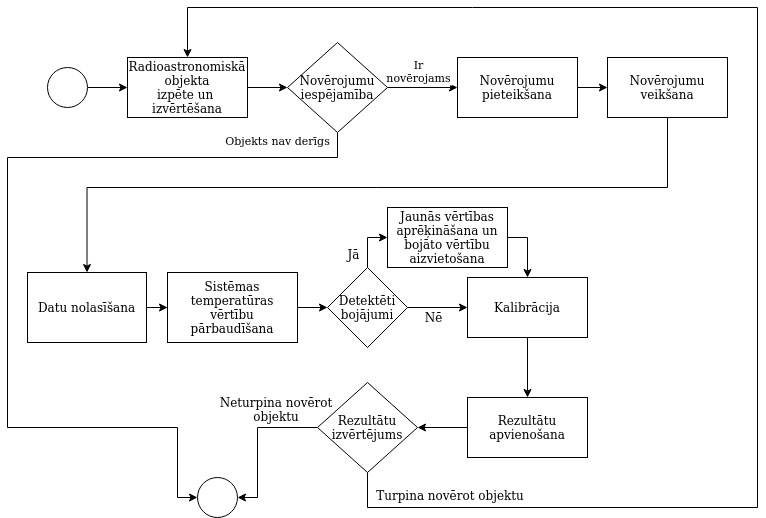
\includegraphics[width=\textwidth]{images/created/workflow-model.png}
\caption{Novērojumu apstrādes metodikas modelis}
\label{fig:workflow}
\end{figure}

%\begin{figure}[htbp]
%  \centering
%    \includesvg[width=\textwidth]{images/created/workflow.svg}
%  \caption{svg image}
%\end{figure}


Bakalaura darba ietvaros tiek aprakstīti visi soļi, izņemot \textit{Novērojumu pieteikšanas} un \textit{Novērojumu veikšanas} soļi, jo minētie soļi ir aprakstīti VSRC un Ventspils Augstskolas nolikumos un iekšējos dokumentos. Visi pārējie soļi aprakstīti pēc sekojošās metodikas - aprakstot teorētisko pamatojumu, realizāciju un iegūtos rezultātus. Radioastronomiskā objekta izpēte un izvērtēšana tiek apskatīta nodaļā \ref{planning}, kur tiek apskatīti raksturlielumi objekta novērošanā, kā arī teorētiskais apraksts novērojumu plānošanai.

Datu nolasīšanas sadaļa aprakstīta nodaļā \ref{read-data}, sistēmas temperatūras pārbaudes aprakstītas anomāliju detektēšana nodaļā \ref{anomalies}, bet pats kalibrācijas process aprakstīts \ref{calibration} nodaļā. Minēto soļu praktisku piemēru var apskatīt \ref{data-process} sadaļā. Novērojumu apvienošanas matemātiskais process aprakstīts \ref{doppler} nodaļā, bet radioastronomisko datu apstrādes rezultātus var apskatīt nodaļā \ref{result-eval}

\section{Novērojuma plānošanas process} \label{planning}



Lai veiktu radioastronmiskā objekta novērošanu, ir jāņem vērā vairāki faktori, kas ietekmēs rezultātu precizitāti un iespējamību. Lai gan turpmāk aprakstītās nodaļas novērojumu veikšanas kritēriji ir svarīgi, jāņem vērā, ka komētu, kuras iespējams detektēt radio frekvenču diapazonā, ir salīdzinoši maz, balstoties uz to, ka komētu OH māzeri izstaro vājus signālus, salīdzinot ar citiem OH māzeriem, līdz ar to ir ieteicams novērot visas komētas, kuras potenciāli detektējamas. Balstoties uz to, ka komētas daļēji sastāv no ledus maisījumiem, novērojumi var sniegt informāciju par ūdeni kosmosā, kā arī ūdens rašanos uz Zemes. Komētu sastāva izpēte sniedz vairāk informāciju komētu zinātniskajai bāzei, tajā skaitā, informāciju par ūdens rašanos uz Zemes, jo komētu sastāvā ir sastopams ūdens ledus formā. 

\begin{wrapfigure}{l}{0.4\textwidth}
    \centering
    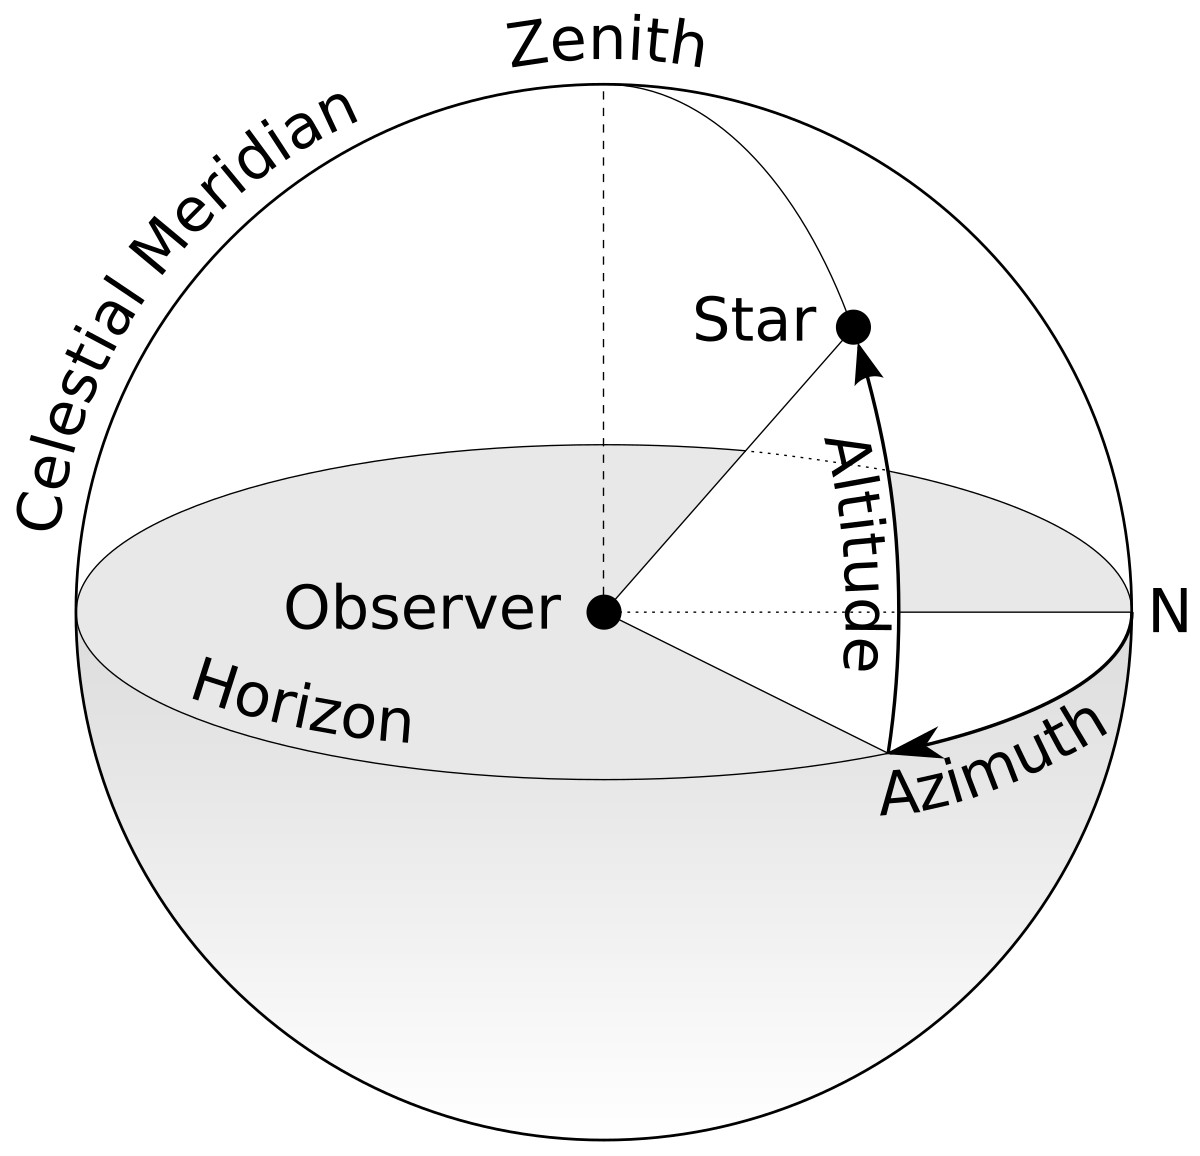
\includegraphics[width=0.4\textwidth]{images/internet/az-el.png}
    \caption{Topocentriskās koordinātu sistēmas attēlojums \cite{az-el-img}}
      \label{fig:az-el}
\end{wrapfigure}
 Par svarīgāko faktoru komētas detektēšanai ar radioteleskopu var uzskatīt objekta pozīciju. Astronomijā tiek izmantota topocentriskā koordināšu sistēma, kurā ir divas neatkarīgas lenķiskās koordinātes - azimuts un elevācija. Sistēma attēlota attēlā \ref{fig:az-el}, kur azimuts - Azimuth, bet elevācija - Altitude. Attēlā, objekts ir zvaigzne, bet zvaigznes vietā var būt jebkurš astronomisks objekts, kurš izstaro radio signālu. Bakalaura darba ietvaros izmantotais Irbenes RT-32 teleskops spējīgs novērot objektus rotējot 360 grādu leņķī, līdz ar to vienīgās vērtības, kuras jāņem vērā, lai novērojums būtu iespējams, ir elevācijas vērtība. Lai gan pēc radioteleskopa lietošanas specifikācijas minimālā elevācijas vērtība ieņem 2.7 grādu vērtību \cite{telescope-spec}, praksē pierādījies, ka elevācijas vērtībām jāpārsniedz 15 grādu robežām, lai iegūtais rezultāts būtu izmantojams, jo objektu novērošana tuvu horizontam nozīmē, ka tiek pastiprināti uztverti apkārtējie radio signālu avoti, kas atrodas uz Zemes virsmas, kā mobilie torņi, Ovīšu bāka un citi. Novērojumu sesijas ilgst vismaz 2 stundas, līdz ar to ir jāpārliecinās, ka elevācijas vērtības ir derīgas visa novērojuma laikā. 
 
 Objekta redzamības grafiku var apskatīt attēlā \ref{fig:swan-el}, kur apskatīts SWAN C/2020 F8 komētas elevācijas vērtības atkarībā no radioteleskopa un objekta pozīcijas no 1. maija līdz 10. maijam, ar sarkanu krāsu iezīmējot potenciāli iespējamos novērojumu laikus.\footnote{Elevācijas vērtības iegūtas no NASA HORIZONS sistēmas} ATLAS komētas redzamības grafiku skatīt pielikumā \ref{fig:atlas-visibility}. Visi grafiki nodaļā tiek izveidoti, izmantojot \textit{Matplotlib Python} bibliotēku \cite{matplotlib}. 

\begin{figure}[H]
\centering
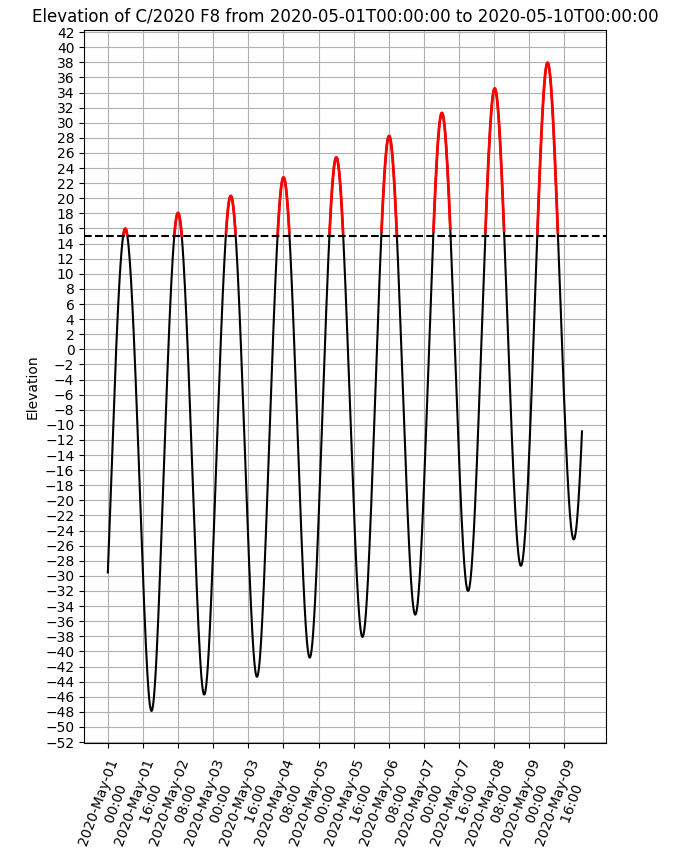
\includegraphics[width=0.75\textwidth]{images/created/swan-smaller.png}
\caption{SWAN C/2020 F8 elevācijas atkarība no laika}

\label{fig:swan-el}
\end{figure}



Veicot vāju radioastronomisku objektu novērojumus, ir nepieciešams novērojuma sesijas laikā novērot arī kādu spēcīgāku avotu jeb kalibratoru, kuru izmanto kontrolei. Tas nozīmē, ka arī kalibratoram ir jābūt redzamam sesijas laikā. Pēdējais nosacījums, objektu novērošanas iespējamībai fiziskā līmenī, ir radioteleskopa noslogojums. Ņemot vērā, ka uz teleskopa izmantošanu ir pieteikušies gan VSRC zinātnieki, gan citu valstu astronomisko institūtu zinātnieki, ir jāņem vērā citu zinātnieku vēlmes un jāplāno savstarpēji vislabākie laiki. 

Komētu datu kvalitāti ļoti ietekmē komētas spilgtums. 
Balstoties uz to, ka komētas aktīvi tiek novērotas optiskajā diapazonā, komētu spilgtums bieži tiek mērīts magnitūdās, pēc kurām iespējams novērtēt komētas spektrālo plūsmas blīvumu novērojumos radio diapazonā. Komētu spilgtumu precīzi noteikt nav viegli, taču izmantojot vairākus avotus, var iegūt aptuveno objekta spilgtumu magnitūdu skaitu. 
Katra magnitūda atbilst 2.512 spilgtuma faktoram, kas nozīmē, ka 1 magnitūdas spilgtuma objekts ir aptuveni 100 reizes spilgtāks par 6 magnitūdas spilgtuma objektu. Bakalaura darba ietvaros tika novērotas komētas, kuru aprēķinātais spilgtums svārstījās robežās no 12 līdz 4 magnitūdām.\footnote{Spilgtuma vērtības iegūtas no NASA HORIZONS sistēmas}

Viens no noteicošajiem faktoriem komētu novērošanas procesā ir komētas pārvietošanās pa tās orbītas. Lai veiksmīgi iegūtu augstas kvalitātes rezultātus, izmantojot patreizējās tehnoloģijas, ir nepieciešams novērot objektu ilgstošā laika periodā. Novērošanas ilgums katrai komētai atšķiras, balsoties uz tās strukturālajiem parametriem un orbītas, pa kuru komēta pārvietojas, taču Bakalaura darba izstrādes laikā, galvenajām novērotajām komētām, minimālais novērojumu laiks bija 110 stundas. Pilnus novērojumu laikus, kā arī citu informatīvo informāciju var apskatīt tabulā  \ref{tab:main-objects}.

Komētai tuvojoties Saulei, palielinās Saules ietekme uz komētu, kas izraisa ķīmiskas reakcijas komētas iekšienē. Komētai ir kodols, kas sastāv no $H_2O$ un papildus ķīmisko elementu piemaisījumiem. Miera stāvoklī kodols ir neaktīvs un sasalis, bet komētai tuvojoties Saulei, Saules ultravioletais starojums ietekmē kodolu. Kodols tiek aktivizēts un tā iekšienē veidojās OH māzeris, kas izstaro OH molekulas. Minēto starojumu ir iespējams novērot radio diapazonā. Kodola aktivitāte ir proporcionāla starojuma spilgtuma jaudai.


Veicot novērojumu, nepieciešams ņemt vērā arī novērotā objekta pozīciju attiecībā pret Zemi. Ņemot vērā, ka OH māzera izstarotais signāls ir salīdzinoši vājš, situācijās, kad komēta ir aktīva, taču atrodas tālu prom no Zemes, nav iespējams objektu novērot citu objektu izstaroto radio starojuma dēļ. Pēc teorijas, radioteleskops spējīgs novērot avotus tūkstošiem astronomisko vienību attālumā, pieņemot, ka avots ir pietiekami spēcīgs. Praksē pierādījies, ka komētām jābūt maksimāli divu astronomisko vienību attālumā no novērošanas punkta, kur komēta, ideālā gadījumā, novietota starp Zemi un Sauli.

Neskatoties uz precīziem skaitļiem, ir jāņem vērā arī komētas popularitāte starp citiem novērotājiem. Jo vairāk astronomi novēro vienu objektu, jo vairāk informācijas pieejama, tādējādi radot iespēju salīdzināt iegūtos rezultātus, kā arī no vairākiem novērojumiem ir efektīvāk iespējams uzzināt objekta aktualitātes. Lai gan pārsvarā astronomi novēro komētas optiskajā diapazonā, rezultāti sniedz informāciju par komētas izmaiņām, piemēram, pateicoties minēto avotu informācijai, bija iespējams detektēt ATLAS Y4/2019 kodola fragmentāciju, kas ļoti ietekmē novērošanas plānus.



%\section{Kopējais process (Workflow)}
\section{Datu nolasīšana} \label{read-data}
% intro
Lai uzsāktu datu apstrādi, ir nepieciešams vispirms izprast datu tipa uzbūvi. Bakalaura darbā tiek apskatīti divi datu tipi, kuri izmantoti komētu novērojumu datu ieguvē un izguvē - jēldati un dat tipa faili. Nodaļā tiks aprakstīta atšķirība starp tiem, kā arī apstrādes process datu izmantošanai.

%novērojumu datu struktūra
%Katrs novērojuma skans ir sadalīts 


% RAW

Katrs novērojuma skans jēldatu gadījumā ir sadalīts astoņās atsevišķās datnēs, kur katrā ir ierakstīts spektrs \textit{int16+int16} reālu un imagināru skaitļu virknē. Lai nolasītu datus, pēc \textit{SDR} spektometra servera dokumentācijas \cite{sdrspec}, Bakalaura darba rakstīšanas laikā visai jēldatu apstrādei papildus Furjē transformācijai, jāizmanto \textit{Blackman-Harris} logošanas funkcija \cite{blackman-harris}, lai iegūtu rezultējošu spektru. Balstoties uz to, ka ieteiktā pārklāšanās robeža \textit{Blackman-Harris} funkcijai ir 66.1\% \cite{overlapping}, tika izveidots algoritms, kas sadala nolasītos datus tvertnēs, kuru garums ir identisks žurnalēšanas failu ierakstītajai \textit{Ns} vērtībai.

Katrai tvertnei tiek izsaukta \textit{Fast Fourier Transform} (turpmāk FFT), kā arī Blackman-Harris funkcija. FFT realizēta, izmantojot \textit{numpy FFT} pakotni \cite{numpy-fft}, bet Blackman-Harris logošanas funkcija izmantojot \textit{scipy signal} pakotni \cite{scipy-blackman}. Pēc FFT veikšanas, tiek apvienotas spektra reālās un imaginārās daļas, un rezultāts ir pieskaitīts kopējai spektru summai. Kad visas datu tvertnes ir apstrādātas, nulles frekvences ir pārvietotas uz vidu un rezultējošais spektrs ir izdalīts ar tvertņu daudzumu, iegūstot vidējo spektru, kas ir skaitļu masīvs ar amplitūdu vērtībām, kuras iegūtas no konkrētā faila. Vizuāli process izklāstīts attēlā \ref{fig:overlapping}, kur attēlots pārklāšanās process izmantojot 75\% pārklāšanās koeficientu. Lai gan attēlā attēlots 75\% pārklāšanās rezultāts, datu apstrāde ar 66.1\% pārklāšanās koeficientu ir ļoti līdzīga, jo mainās tikai kopējais spektru daudzums.

\begin{figure}[H]
\centering
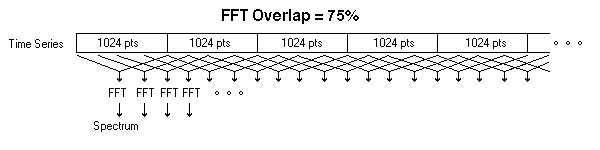
\includegraphics[width=\textwidth]{images/internet/OVERLAP2.png}
\caption{Furjē transformācijas pielietojums uz datu tvertnēm ar 75\% pārklāšanās koeficientu. \cite{overlapping-img}}
\label{fig:overlapping}
\end{figure}

% DAT
Dat formāta datu gadījumā, dati jau ir apstrādāti ar iepriekš minētajām funkcijām, līdz ar to tie ir ierakstīti \textit{CSV} tipa failā trijās kolonnās. Pirmajā kolonnā ierakstītas frekvenču joslas vērtības konkrētajām amplitūdām, otrajā kolonna ierakstītas kreisās cirkulārās polarizācijas amplitūdu vērtības, bet trešajā ierakstītas labās cirkulārās polarizācijas amplitūdu vērtības. Tā kā abas polarizācijas ir saglabātas vienā failā, kopējais failu daudzums vienam skanam ir četri.

Kopējais failu skaits novērojumā atkarīgs no novērojuma ilguma, taču katram failam nav precīza ierakstīšanas ilguma. Četru stundu novērojumiem kopā ir 240 skani, bet divu stundu novērojumiem 120. Balstoties uz minēto informāciju, var detektēt situācijas, kur novērošanas sesijā bijušas tehniskas problēmas, jo patiesais failu daudzums neatbilst plānotajam, un izvērtēt, vai datus izmantot.

Lai gan dat formāta failu rezultāti ir neprecīzāki par jēldatu failu rezultātiem, tie tiek biežāk izmantoti sava ērtuma dēļ, jo bieži tiek apskatīti spēcīga signāla objekti un noklusējuma konfigurācija tiem ir apmierinoša. Priekšrocība jēldatiem ir to konfigurēšanas iespējas, taču jāņem vērā, ka to apstrādei nepieciešami vairāk skaitļošanas un laika resursi. Novērojot objektus un rezultātus ierakstot jēldatu formātā,  nepieciešama salīdzinoši liela datu krātuve, jo divu stundu novērojums atbilst aptuveni 340 gigabaitiem atmiņas, kamēr dat tipa failu novērojumi aizņem tikai ap 70 megabaitiem.

Lai izvērtētu datu apstrādes veiktspēju, tiek veikti veiktspējas testi, kuri aprakstīti \ref{algorithm-eval} nodaļā, kur apskatīts gan pirmās iterācijas, gan pēdējās iterācijas algoritmu izpildes laiks, kā arī procesu daudzuma ietekme uz pēdējās iterācijas algoritma izpildes laiku. Algoritma realizāciju var apskatīt pielikumā \ref{appendix:codes}.

% comparison?
%Nodaļai nevar būt tikai viena apakšnodaļa. Analītiskās daļas  uzdevums ir sistematizētā veidā sniegt pētāmās problēmas īsu teorētisku pamatojumu, autora pētījuma rezultātus, kas formulēti priekšlikumu veidā. Visās analītiskās daļas nodaļās (izņemot teorētisko pamatojumu) jābūt ilustratīvajam materiālam un aprēķiniem: konkrētiem plāna aprēķiniem, analītiskām tabulām, diagrammām u.tml.


\section{Kalibrācijas process} \label{calibration}

%pamatojums, kāpēc kalibrācija ir nepieciešama

% galvenās darbības kaliobrācijas procesā
%% formulas arī
%piezīmei par kalibrācijas uzlabojumi tiks apskatītiti ndoaļa 3.2.xxx

Nodaļā aprakstītas kalibrācijas procesā izmantotās formulas, taču ņemot vērā, ka Bakalaura darba mērķis ir orientēts uz algoritmisko izpildi, nevis fizikālo pamatojumu, formulu izmantošanas pamatojums netiek sniegts. Aprakstītā kalibrācijas metode tiek izmantota spēcīgu māzeru novērojumos, līdz ar to, pamatalgoritms ir ticis izveidots jau iepriekš, ņemot par pamatu citās radio stacijās izmantotos kalibrēšanas algoritmus.

Kalibrācijas process ir izveidots, izmantojot rakstu \textit{Unbiased flux calibration methods for spectral-line radio observations} \cite{unbiased}, kurā aprakstītas metodes efektīvai datu kalibrācijai - pozīciju maiņa un frekvenču maiņa. Pozīciju maiņā teleskops tiek norādīts uz references pozīciju pirms tas tiek pozicionēts uz novērojumu objektu.
Frekvenču maiņas metodē, tiek izmantoti divi lokālie oscilatori, kur viens no tiem tiek izmantots, lai sniegtu atskaites spektru. Veicot novērojumus teleskopa stars netiek fiziski bīdīts prom no avota, līdz ar to, nav iespējams veikt pozīciju maiņas pieeju, tāpēc tiek izmantota frekvenču maiņas metode.

Frekvenču maiņas metodes rezultātā veidojas 4 dažādas fāzes - $P_{off}^{sig}$, $P_{on}^{sig}$, $P_{off}^{ref}$, $P_{on}^{ref}$. Šie apzīmējumi tiek izmantoti formulās \eqref{eq:1.2.1}, \eqref{eq:1.2.2}, \eqref{eq:1.2.3}, \eqref{eq:1.2.4}, \eqref{eq:1.2.5} un \eqref{eq:1.2.6},
kur: 
\begin{tabbing}
\phantom{\hspace{10mm}}\= \kill
$P_{off}^{sig}$\> = Lokālā oscilatora ierakstītais signāls ar izslēgtu trokšņa diodi\\
$P_{on}^{sig}$\>   = Lokālā oscilatora ierakstītais signāls ar ieslēgtu trokšņa diodi\\
$P_{off}^{ref}$\>   = References lokālā oscilatora ierakstītais signāls ar izslēgtu trokšņa diodi\\
$P_{on}^{ref}$\> = References lokālā oscilatora ierakstītais signāls ar ieslēgtu trokšņa diodi\\
\end{tabbing}

Lai iegūtu datus par objekta plūsmas blīvumu, ir jāņem vērā kopējā sistēmas trokšņa temperatūra pēc formulas \ref{eq:1.2.1}. 

\begin{equation}
T_{sys}^{[cal]} = T_{bg} + T_{atm} + T_{atm} + T_{spill} + T_{loss} + T_{rx} + T_{cal} \tag{1.2.1}\label{eq:1.2.1} 
\end{equation}
kur: 
\begin{tabbing}
\phantom{\hspace{10mm}}\= \kill
$T_{sys}^{[cal]}$\> = Kopējā sistēmas trokšņa temperatūra \\
$T_{bg}$\> = Mikroviļņu un galaktiskā fona troksnis \\
$T_{atm}$\> = Atmosfēras troksnis \\
$T_{spill}$\> = Zemes virsmas troksnis \\
$T_{loss}$\> = Novērojumā zaudētā informācija \\
$T_{rx}$\> = Uztvērēja trokšņa temperatūra \\
$T_{cal}$\>   =  Injicētais troksnis, izmantojot trokšņa diodi\\
\end{tabbing}



Taču visas minētās vērtības iegūt nav vienkārši, līdz ar to tiek piedāvāts alternatīvs veids, kā aprēķināt sistēmas temperatūru no iegūtajiem datiem. Ja $T_{sys}^{off}$ un $T_{cal}$ tiek uzskatītas par konstantēm attiecībā pret laiku un frekvenci, iegūst vienādojumus:
%Eq25
\begin{equation}
T_{sys,ref}^{off} = T_{cal} \frac{ \left( P_{on}^{ref} + P_{off}^{ref} \right)  -  \langle P_{on}^{ref} - P_{off}^{ref} \rangle_v }{2 \langle  P_{on}^{ref} - P_{off}^{ref} \rangle} \tag{1.2.2}\label{eq:1.2.2} 
\end{equation}
kur: 
\begin{tabbing}
\phantom{\hspace{30mm}}\= \kill
$\langle P_{on}^{ref} - P_{off}^{ref} \rangle_v$\> = References oscilatora spektru starpības iekšējo 50 \% vidējā vērtība\\
$T_{cal}$\>   =  Injicētais troksnis, izmantojot trokšņa diodi\\
$T_{sys,ref}^{off}$\> = Sistēmas temperatūra izslēgtai trokšņa diodes references oscilatora signālam\\
\end{tabbing}

\begin{equation}
T_{sys,sig}^{off} = T_{cal} \frac{ \left( P_{on}^{sig} + P_{off}^{sig} \right)  -  \langle P_{on}^{sig} - P_{off}^{sig} \rangle }{2 \langle  P_{on}^{sig} - P_{off}^{sig} \rangle} \tag{1.2.3}\label{eq:1.2.3} 
\end{equation}
\begin{tabbing}
\phantom{\hspace{30mm}}\= \kill
$\langle P_{on}^{sig} - P_{off}^{sig} \rangle_v$\> = Lokālā oscilatora spektru starpības iekšējo 50 \% vidējā vērtība\\
$T_{cal}$\>   = Injicētais troksnis izmantojot trokšņa diodi\\
$T_{sys,sig}^{off}$\>  = Sistēmas temperatūra izslēgtai trokšņa diodes lokālā oscilatora signālam\\
\end{tabbing}
%EQ:24
%\begin{equation}
%\frac{T_{sys,off}}{T_{cal}} \approx \frac{(P_{off}^{cal}+P_{off}) - \langle P_{off}^{ref} - P_{off}^{ref}\rangle_v }{2 \langle  P_{off}^{cal}-P_{off} \rangle_v }
%\end{equation}





%EQ27:

%\[T_{sou} = \overline{T}_{sys,off} \frac{P_{on} - P_{off}{4} \]

%article formula:
%\[ T_{sou} = \overline{T}_{sys,off} \frac{P_{on}-P_{off}}{P_{off}} = \left( \overline{T}_{sys,off} + T_{cal} \right) \frac{P_{on}^{cal} - P_{off}^{cal}}{P_{off}^{cal}} \]

Izmantojot skalāru $T_{cal}$ vērtību, zināmu katram uztvērējam, var iegūt kalibrētu spektru izslēgtai trokšņa diodei:

\begin{equation}
T_{cal,ref}^{off} = T_{sys,ref}^{off} \cdot \frac{(P_{off}^{sig} - P_{off}^{ref})}{P_{off}^{ref}}\tag{1.2.4}\label{eq:1.2.4} 
\end{equation}
kur:
\begin{tabbing}
\phantom{\hspace{20mm}}\= \kill
$T_{sys,ref}^{off}$\>  = Sistēmas temperatūra izslēgtai trokšņa diodes references oscilatora signālam\\
$T_{cal,ref}^{off}$\>  = Kalibrētas sistēmas temperatūra izslēgtai trokšņa diodes references oscilatora \\ signālam\\
\end{tabbing}
\begin{equation}
T_{cal,sig}^{off} = T_{sys,sig}^{off} \cdot \frac{(P_{off}^{ref} - P_{off}^{sig})}{P_{off}^{sig}}\tag{1.2.5}\label{eq:1.2.5} 
\end{equation}
kur:
\begin{tabbing}
\phantom{\hspace{20mm}}\= \kill
$T_{sys,sig}^{off}$\>  = Sistēmas temperatūra izslēgtai trokšņa diodes lokālā oscilatora signālam\\
$T_{cal,sig}^{off}$\>  = Kalibrētas sistēmas temperatūra izslēgtai trokšņa diodes lokālā oscilatora \\ signālam\\
\end{tabbing}

Līdz ar to, lai aprēķinātu sistēmas temperatūru ieslēgtai trokšņa diodei, papildus jāapskata trokšņa diodes temperatūra. 
%34

\begin{equation}
T_{cal,ref}^{on} = \left( T_{sys,ref}^{off} + T_{cal} \right) \cdot \frac{\left( P_{on}^{sig} -  P_{on}^{ref}\right)}{ P_{on}^{ref}}\tag{1.2.6}\label{eq:1.2.6}   
\end{equation}

\begin{equation}
T_{cal, sig}^{on} = \left( T_{sys,sig}^{off} + T_{cal} \right) \cdot \frac{\left( P_{on}^{ref} -  P_{on}^{sig}\right)}{ P_{on}^{sig}}\tag{1.2.7}\label{eq:1.2.7}  
\end{equation}
kur:
\begin{tabbing}
\phantom{\hspace{20mm}}\= \kill
$T_{cal,ref}^{on}$\>  = Rezultējošā sistēmas temperatūra lokālā oscilatora references signālam\\ ieslēgtai trokšņa diodei\\
$T_{cal,sig}^{on}$\>  = Rezultējošā sistēmas temperatūra lokālā oscilatora signālam ieslēgtai \\ trokšņa diodei\\
$T_{sys,ref}^{off}$\>  = Kalibrētas sistēmas temperatūra izslēgtai trokšņa diodes lokālā oscilatora \\ signālam izslēgtai trokšņa diodei\\
$T_{sys,ref}^{off}$\>  = Kalibrētas sistēmas temperatūra izslēgtai trokšņa diodes lokālā oscilatora \\references signālam \\
$T_{cal}$\>  = Injicētais troksnis, izmantojot trokšņa diodi\\


\end{tabbing}

%\[ T_{sou,-} - T_{sou,+} + \Delta T_{sys,\pm}^{[cal]} = \left( T_{sou,-} + T_{sys,-}^{[cal]}  \right) \frac{P_{ref}^{[cal]}-P_{ref}^{[cal]}}{P_{sig}^{[cal]}} \equiv \Tilde{T}_{ref}^{[cal]} \]

Spektri ir apvienoti, lai gala rezultātā samazinātu troksni:

\begin{equation}
T_{cal}^{sig} = \frac{T_{cal, sig}^{on} + T_{cal, sig}^{off}}{2} \tag{1.2.8}\label{eq:1.2.8} 
\end{equation}

\begin{equation}
T_{cal}^{ref} = \frac{T_{cal, ref}^{on} + T_{cal, ref}^{off}}{2}\tag{1.2.9}\label{eq:1.2.9} 
\end{equation}


Lai iegūtu optimālu rezultātu $T_{rez}$ vērtības, ir arī jāveic frekvenču pārvirzīšana, bet Bakalaura darba ietvaros tiek izmantota \textit{ numpy roll } funkcija, kurai tiek padots $T_{rez}$ spektrs, kā arī pārbīdes koeficients. Rezultējošie spektri tiek apvienoti:
\begin{equation}
T_{rez} = \frac{T_{cal}^{sig} + T_{cal}^{ref}}{2}\tag{1.2.10}\label{eq:1.2.10} 
\end{equation}


Rezultāti tiek pārveidoti no kelviniem uz janskijiem, lai efektīvāk attēlotu plūsmas blīvumu. Jāņem vērā Zemes atrašanās vieta attiecībā pret objektu, līdz ar to tiek rēķinātas vērtības polinoma vērtības Zemes atrašanās vietā. Tas tiek darīts pēc formulas:

\begin{equation}
Sf = \frac{T_{rez}}{ DPFU \cdot f(Gel,El))}\tag{1.2.11}\label{eq:1.2.11} 
\end{equation}
kur:
\begin{tabbing}
\phantom{\hspace{30mm}}\= \kill
$Sf$\>  = Rezultējošais spektrālās plūsmas blīvums\\
$T_{rez}$\>  = Rezultējošā sistēmas temperatūra\\
$DPFU$\>  = (Degree per flux unit) Grādi uz plūsmas vienību\\
$f(Gel,El))$\>  = Aprēķinātā elevācijas polinoma vērtība \\
\end{tabbing}

Nodaļā aprakstītās formulas tiek pielietotas divreiz, katrai polarizācijai.
Kalibrācijas rezultātā tiek iegūts plūsmas blīvuma spektrs, kurš attēlo enerģiju, kas iegūta attālumā no novērotā objekta laukuma, kurš atrodas novērojuma brīdī veiktajā attālumā starp radioteleskopu un novēroto objektu. Algoritma implementāciju var apskatīt pielikumā \ref{appendix:codes}.



\section{Doplera kompensācija un objekta pārvietošanās ātruma aprēķins} \label{doppler}
Nākamais solis vāju radioastronomisku objektu novērojumu procesā ir vairāku novērojumu apvienošana. Ņemot vērā, ka katrā novērojuma iterācijā stohastiskais troksnis dod signālam dažādas vērtības, apvienojot vairākus novērojumus, stohastiskais troksnis samazināsies ar katru iterāciju, bet novērojuma objekta vērtības nemainīsies.  Lai to realizētu, ir jāņem vērā faktors, ka gan novērotais objekts, gan Zeme pārvietojas Saules sistēmā. Tas nozīmē, ka rezultējošo novērojuma frekvenci ietekmēs Doplera efekts un iegūtais frekvenču masīvs ir jāmodificē, lai pārbīde tiktu ņemta vērā. 

Doplera efekta aprēķins ir atšķirīgs, atkarībā no objekta atrašanās vietas. Ņemot vērā to, ka Bakalaura darba ietvaros, tika apskatīti gan Saules sistēmas objekti, gan maiņzvaignes un māzeri ārpus Saules sistēmas, tika izpētītas atšķirīgās pieejas nobīdes aprēķinam. Lai aprēķinātu Doplera efektu objektiem ārpus Saules sistēmas, ir nepieciešams zināt objektu pārvietošanās ātrumu. Tā kā novērotos radioastronomiskos objektus ārpus Saules sistēmas var uzskatīt par punktveida objektiem, visa ātruma vektoru ietekme tiek aprēķināta ar formulu:
\begin{equation}
V_{total} = (V_{sun} + V_{obs} + V_{Earth}) \tag{1.3.1}\label{eq:1.3.1} 
\end{equation}
kur: 
\begin{tabbing}
\phantom{\hspace{10mm}}\= \kill
$V_{total}$\> = Rezultējošais objekta ātrums \\
$V_{sun}$\>   = Vidējais Saules pārvietošanās ātrums novērojuma laikā\\
$V_{obs}$\>   = Vidējais objekta ātrums novērojuma laikā\\
$V_{Earth}$\> = Vidējais Zemes pārvietošanās ātrums novērojuma laikā\\


\end{tabbing}



Lai iegūtu rezultējošās objekta pārvietošanās ātruma vērtības, tika izmantots jau eksistējošs programrisinājums, kas tika radīts radioastronomisku māzeru novērojumiem.\cite{vlsr} %mention RA/DEC? 
Metode izmanto māzera spektrālo līniju pīķus, lai iegūtu rezultējošo ātrumu pēc formulas:


\begin{equation}
V_{rez}=\left(\frac{f_{obs}}{f_{rest}}-1 \right) \cdot c + V_{total} \tag{1.3.2}\label{eq:1.3.2} 
\end{equation}
kur: 
\begin{tabbing}
\phantom{\hspace{10mm}}\= \kill
$V_{rez}$\> = Rezultējošais ātruma masīvs, attiecīgajai frekvencei \\
$f_{obs}$\>   = Novērojumā iegūtā frekvenču josla\\
$f_{rest}$\>   = OH molekulu spektrālo līniju frekvence \\
$c$\> = Gaismas ātrums\\
$V_{total}$\> = Objekta rezultējošais pārvietošanās ātrums (skat. \eqref{eq:1.3.1} formulu) \\\\

\end{tabbing}

Ķermeņus Saules sistēmā nevar uzskatīt par punktveida objektiem, jo ātruma vektoru ietekme uz objektu ir lielāka. Lai iegūtu radioastronomiskā objekta ātrumu, ir iespējams izmantot Keplera orbitālos parametrus \cite{kepler-elements}, taču lai atvieglotu darbu, kā arī mazinātu kļūdu iespējamību, tiek izmantota NASA HORIZONS sistēma \cite{horizons}, kura uzglabā lielu daudzumu informācijas par Saules sistēmas objektiem, to skaitā, objektu atrašanās vietu konkrētos laikos, kā arī objektu ātrumu konkrētajā laikā. Iegūtais ātrums novērojuma laika periodā tiek ievietots \eqref{eq:1.3.2} formulas $V_{total}$ mainīgajā.


Novērojumu veikšanas laikā, Doplera pārbīde jau tiek ņemta vērā, izmantojot aprakstīto metodiku, taču esošais algoritms paredzēts mazāka joslas platuma novērojumos, līdz ar to tiek izmantots vidējais ātrums visā novērojumā. Ņemot vērā minēto faktoru, spektrs tiek pārbīdīts atpakaļ par nobīdīto vērtību, sadalīts uz pusēm, kur pirmā puse reprezentē 1665MHz frekvences diapazona spektru, bet otra puse - 1667MHz frekvences diapazona spektru, katrai daļai pārrēķinātas ātruma vērtības un attiecīgi pārbīdītas. Pareizā pārbīde tiek rēķināta pēc formulas:


\begin{equation}
df  = f_0 - \frac{f_0}{1- \frac{V_{object}}{c}}
\tag{1.3.3}\label{eq:1.3.3} 
\end{equation}
kur: 
\begin{tabbing}
\phantom{\hspace{15mm}}\= \kill
${df}$\> = Aprēķinātā spektra nobīde \\
$f_{0}$\>   = Novērojumā iegūtā frekvenču josla\\
$c$\> = Gaismas ātrums\\
$V_{object}$\> = Objekta radiālais ātrums relatīvs uztvērēja antenai \\\\

\end{tabbing}





%vel = rezultējošais ātruma masīvs

%f_obs = frekvenču masīvs, kurš iegūts kalibrācijas rezultātā

%f_rest = rest frekvence (1.665402 vai 1.6673590) 

%c = gaismas ātrums

%v_sun = vidējais saules ātrums? vai šis būtu VmagSn no HORIZONS? (Magnitude of target center velocity with respect to the Sun)

%v_obs = objekta ātrums? vai šis būtu VmagOb no HORIZONS?

%v_earth = vidējais zemes ātrums?

%v_total = ātrums, kuru lieku iekšā doplera funkcijā

%Piemēra rezultāti uz atlas 0:

%v_sun:  5.3263164389446

%v_obs:  0.08472007198849721

%v_earth:  -15.215724915542548

%v_total:  -9.80468840460945




\section{Veivletu izmantošana radioastronomisku signālu apstrādē} \label{wavelets}
\subsection{Veivletu definēšana}
%pamatojuma daļā aprakstīt, ka veicletu teoretiskā ... netik plai izklāštīts, bet galvenasi uzsvars ir uz to izmantošanutiek izmantoti
Lai precīzāk analizētu signālus ar pēkšņām pārmaiņām, ir nepieciešams izmantot netradicionālākas metodes par Furjē transformāciju, kas reprezentē signālu kā sinosoīdu summu, kas nav lokalizēta laikā vai telpā. Lai veiktu signālu apstrādi, tika izmantota jauna funkciju klase – veivleti.  

Veivlets ir viļņveida svārstība ar amplitūdu, kas sākas ar nulli, palielinās vai samazinās un gala rezultātā atgriežas nulles vērtībā. Veivletiem ir dažādi tipi un grupējumi, un tos arī iedala pēc īpašībām, taču tiem ir vienots nosacījums -  veivleta amplitūdas vidējā vērtība ir nulle. Veivletu plašais formu klāsts ir viens no galvenajiem iemesliem veivletu izmantošanai signālu apstrādē. Lai vieglāk grupētu veivletus, tie ir iedalīti vairākās ģimenēs, taču konkrētie veivleti ir tikai visbiežāk izmantotie – veivletus var veidot jebkurš, ja vien izveidotais atbilst kritērijiem. 


Viena no veivletu transformācijas formām ir diskrētā vievletu transformācija, kura visbiežāk tiek izmantota datu trokšņa samazināšanā un datu kompresijā. Process ir līdzīgs signāla salīdzināšanai ar filtru bankām. Diskrētā veivletu transformācija attēlota attēlā \ref{fig:wavelets-dwt}, kur modelēts apstrādes process.

\begin{figure}[h!]
\centering
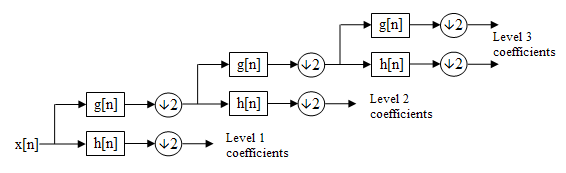
\includegraphics[width=\textwidth]{images/internet/DWT-fig.png}
\caption{Diskrētās veivletu transformācijas vizuālais attēlojums} \cite{dwt-fig}
\label{fig:wavelets-dwt}

\end{figure}



Signāls tiek filtrēts, izmantojot \textit{low-pass} un \textit{high-pass} filtrus, lai iegūtu \textit{low-pass} jeb aproksimācijas koeficientu, un \textit{high-pass} jeb detaļu koeficientu apakšjoslas. Nākamajā dekompozīcijas līmenī, \textit{low-pass} apakšjosla, tiek iteratīvi filtrēta, izmantojot to pašu metodi, kuru sākuma signāls. Koeficientu daudzums katrā apakšjoslā ir puse no koeficientiem no iepriekšējās apakšjoslas. 


Lai gan veivletiem ir vairākas metodes, kā tos pielietot signāla trokšņa samazināšanai, Bakalaura darba ietvaros tika izmantota veivletu sliekšņošna. Ir apskatītas diva veida slieksņošanas operācijas – mīkstā un cietā. Abos gadījumos koeficientiem ar vērtībām zem noteiktā sliekšņa tiek piešķirta vērtība nulle, bet atšķiras, kas notiek ar pārējiem koeficientiem. Mīkstajā metodē koeficienti, kas lielāki par norādīto slieksni ir samazināti, atņemot sliekšņa vērtību no koeficienta vērtības, taču cietajā – koeficienti paliek nemainīgi. Bakalaura darba ietvaros pēc noklusējuma tiek izmantota mīkstā sliekšņošanas metode, jo metodes pielietojums bija piemērotākā uzdevumu veikšanai.
%Vizuāli attēlojot šo procesu un apzīmējot high-pass apakš joslu ar h[n] un low-pass apakš joslu ar g[n], iegūst Ilustrāciju 1.  

%[bilde]



\subsection{Veivletu pielietojums}

Veivletu transformācija Bakalaura darba ietvaros tika realizēta izmantojot \textit{PyWavelets} \cite{pywt} Python bibliotēku. Bibliotēka tika izvēlēta, tās atvieglotās veivletu transformācijas realizācijas dēļ, kā arī plašo iebūvēto veivletu dēļ. Pēc noklusējuma tiek atbalstīti 106 veivleti, kuri atbalsta diskrēto veivletu transformāciju no sekojošām ģimenēm - bior, coif, db, dmey, haar, rbio, sym.

Plašo konfigurēšanas iespēju dēļ, veivletu pielietošana tika testēta gandrīz visos datu apstrādes procesos, ar atšķirīgu efektivitāti. Pielietojot šāda veida transformāciju, jāņem vērā, ka ar katru transformāciju, tiek zaudēti ar vien vairāk dati. Tas nozīmē, ka, ja transformācija tiks izmantota pārāk daudz, var tikt zaudētas spektra detaļas, kuras sākotnēji būtu redzamas. Arī jāņem vērā, ka iegūtais spektrs ir balstīts uz paša veivleta formu, līdz ar to, var rasties situācijas, kur veivlets izceļ pīķi konkrētā vietā, taču tas nav meklētais signāls. Problēma tiek novērsta salīdzinot vairāku veivletu iegūtos rezultātus savā starpā, jo, ja vairākas formas veivletu spektri iegūst pīķi vienādās frekvences vērtībās, var uzskatīt, ka tā nav sagadīšanās.

\begin{figure}[h!]

\centering
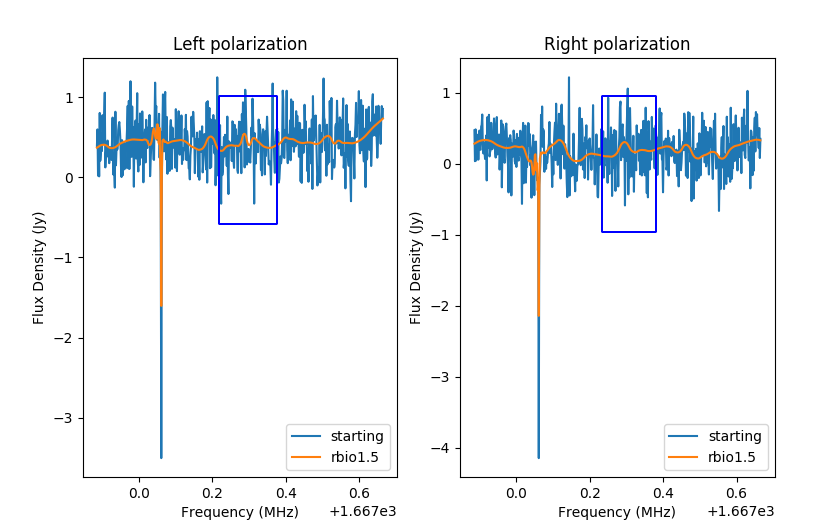
\includegraphics[width=\textwidth]{images/created/rbio15-rlmi-sdr-boxed.png}
\caption{Pirmie iegūtie rezultāti uz R Leonis Minoris izmantojot rbio1.5 veivletu ar 0.5 slieksni}
\label{fig:rlmi-boxed}
\end{figure}


Veivletu transformācijas pielietojuma iespējas ir ļoti plašas augstās konfigurēšanas iespējas dēļ, jo ir iespējams izmantot visus 106 iebūvētos veivletus un tiem norādīt savu precizitātes koeficientu, kā arī sliekšņošanas tipu. Tas nozīmē, ka katrs veivlets var tikt pielietots datiem, bet atkarībā no pielietotā veivleta rezultāts būs labāks vai sliktāks. Bakalaura darba pētījuma laikā tika atrasti vairāki veivleti, kurus iespējams efektīvi izmantot visos apskatītajos gadījumos.



Veivletu pielietošana Bakalaura darba ietvaros aizsākās ar mērķi novērst stohastisko troksni pirms vairāku novērojumu apvienošanas. Izmantojot veivletus, bija iespējams detektēt pirmās pazīmes maiņzvaigznes R Leonis Minoris OH māzera novērošanā, kuras attēlotas attēlā \ref{fig:rlmi-boxed}. Grafikā attēlota plūsmas blīvuma attiecība pret frekvenci, kur, izmantojot sākotnējo signālu, ir izveidots jauns spektrs izmantojot rbio1.5 veivletu ar 0.5 slieksni. Zilajā četrstūrī ir iezīmēts potenciāli novērotais OH māzera plūsmas blīvums, kurš, lai gan, nevar būt uzskatīts par detektētu signālu balstoties uz 3 sigmu likuma, sniedz informāciju, ka novērojot objektu ilgāku laiku būs iespējams iegūt detektējamu signālu. Lai gan apstrādes metodika ir mainījusies, darbs ar veivletiem ir atvēris vairākas iespējas datu apstrādes patreizējā metodikā gan \ref{anomalies} nodaļā aprakstītajā anomāliju detektēšanā, gan stohastiskā trokšņa mazināšanu komētu datu apstrādes rezultātiem.






%\section{Vāju radioastronomisko objektu novērojumu programmrisinājumu}
\section{MPI integrācija kalibrācijas procesā}

Balstoties uz to, ka jēldatu apstrādes process ir laikietilpīgs, kā arī resursietilpīgs process, to ir nepieciešams efektīvi paralelizēt. Veids, kā tas tiek darīts Bakalaura darba datu apstrādes sistēmā, ir, izmantojot \textit{Python} bibliotēkas \textit{mpi4py} \cite{mpi-docs} iespējas, kura realizē \textit{Message Passing Interface} jeb \textit{MPI} protokolu python valodā, kas atļauj \textit{Python} procesam izmantot vairākus kodolus vienlaicīgi.

Lai testētu \textit{MPI} integrāciju kalibrācijas procesā, tika izveidots programrisinājums, kurš paredzēts izmantošanai ar deviņiem \textit{MPI} procesiem, kur process nr. 1  atbild par failu apstrādes organizēšanu un masīvu apstrādi, bet procesi 2-9 veic jēldatu nolasīšanu, kura aprakstīta nodaļā \ref{read-data} Izpildes procesa piemērs attēlots pielikumā \ref{appendix:old-version}, kur pa soļiem attēlota datu apstrādes loģika un informācijas plūsma. Procesi attēloti, kā apļi, kuru centrā norādīts fails, kurš patreiz tiek apstrādāts.

%Process 0 sākotnēji nolasa visus jēldatus direktorijā, tad katrus 8 failus sūta savam procesam. Šie procesi nolasa datus un rezultējošo masīvu atsūta atpakaļ procesam 0, kas uzsāk kalibrācijas procesu. Kad kalibrācija ir pabeigta un jaunais rezultāts ir saglabāts, process cikliski atsākas nākamajiem 8 failiem, līdz apstrādāti visi dati. Kad visi dati nolasīti, process 0 nosūta pārējiem procesiem informāciju par datu apstrādes beigām un šie procesi pārstāj darbību.

Ņemot vērtā to, ka sākotnējā MPI algoritma versija bija spējīga izmantot tikai 9 procesus datu apstrādei, bet pieejami bija daudz vairāk skaitļošanas resursu, algoritms tika pilnībā pārveidots. Algoritma versija Bakalaura nodošanas laikā spējīga datus apstrādāt neierobežotā kodolu skaitā, pilnvērtīgi izmantojot visus iedalītos kodolus.

Algoritma process nr. 1 uzlabotajā algoritmā atbild par kalibrēšanu un datu apvienošanu. Process nr. 2 - par pārējo procesu pārvaldību un failu nosaukumu nodošanu pārējiem procesiem. Procesam ar numuru 3 ir iedalīts speciāls uzdevums - nokalibrēt dat failus, jo dat failu apstrādes process ir ļoti ātrs un lietotāja ērtības dēļ, visas darbības tiek koncentrētas vienotā algoritmā. Kad process nr. 3 ir nokalibrējis dat failus, tas tiek pievienots pārējiem, jēldatu nolasīšanai paredzētajiem, procesiem. Tas nozīmē, ka algoritmu ir nepieciešams startēt, izmantojot vismaz 3 procesus, lai gan algoritms paredzēts daudz vairāku procesu izmantošanai. Izpildes procesa piemērs attēlots pielikumā \ref{appendix:new-version}, kur attēlota procesu komunikācija un datu apstrādes process. Kā piemērs, tiek apskatīts potenciālā komunikācija starp astoņiem procesiem, taču līdzīgs rezultāts ir iegūstams jebkurā procesu daudzumā. Jāņem vērā, ka katrā algoritma izpildes reizē komunikācija var atšķirties, jo nolasīšanas ātrums nav konstants. Procesi pielikumā \ref{appendix:new-version} attēloti kā apļi, kuru centrā norādīts procesa pieejamības stāvoklis.

Process nr. 2 ir algoritma sarežģītākā daļa, jo ir nepieciešams nodrošināt, ka visiem iedalītajiem procesiem vienmēr ir iedalīts savs fails un iedalītais process strādā pie faila nolasīšanas, kā arī jānodrošina, ka visi dati ir apstrādāti. Tas tiek realizēts ar masīvu, kur katrs elements atbilst procesa statusam. Sākotnēji procesu vērtības inicializētas ar vērtību 1, izņemot pirmās 3, jo minētie procesi jau ir aizņemti.
Tad process, ciklā visu failu sarakstam, sūta failu ceļu pirmajam procesam, kurš ieņēmis stāvokli "1". Ja faila ceļš nosūtīts, atbilstošais procesa statuss attiecīgi ir mainīts uz 0, lai attēlotu, ka tas ir aizņemts. Ja visi procesi ir aizņemti, process 2 gaida uz kādu no pārējiem procesiem, lai tas nosūtītu apstiprinošu ziņu, ka dati nolasīti un iedala attiecīgajam procesam jaunu failu apstrādei. Kad visi faili nolasīti, pārējiem procesiem tiek aizsūtīta ziņa par datu apstrādes beigām un procesi apkopo savus datus vienā datu struktūrā, kuru nosūta procesam 1 tālākai apstrādei.  

Algoritmam tika veikti veiktspējas testi, kuri aprakstīti \ref{algorithm-eval} nodaļā. Tiek apskatītas atšķirības no vecā algoritma versijas veiktspējas, kā arī fināla versijas algoritma veiktspējas atkarība no kodolu daudzuma.




%\section{Stoka parametri (Varbūt neizmantos)}
%Lai nodrošinātu datu integritāti, tika apskatīti arī datu Stoka parametri - vērtību kopa, kas apraksta polarizācijas radiācijas stāvokli. Balstoties uz rakstu par Nançay radioastronomijas observatorijas iegūtajiem rezultātiem no 2007-2009 gada \cite{nancay}, kurā tika aprakstīta informācija par laika periodā novērotajām maiņzvaigznēm, bija iespējams salīdzināt šos rezultātus ar bakalaura darba laikā apskatītā objekta rezultātiem. 


%Bakalaura darba ietvaros, tika izpētīts \textit{The Measurement of Polarization in Radio Astronomy} \cite{stokes} raksts, lai iegūtu formulas cirkulārās polarizācijas Stokes parametru aprēķinam:
%\begin{equation}
%I= \langle E_R^2 \rangle + \langle E_L^2 \rangle \tag{2.2.5.1}\label{eq:2.2.5.1}
%\end{equation}
%\begin{equation}
%Q = 2 \langle Re(E_R E_L^*) \rangle = 2 \langle E_R E_L \cos{\delta_{RL}} \rangle \tag{2.2.5.3}\label{eq:2.2.5.3}
%\end{equation}
%\begin{equation}
%U = 2 \langle Im(E_R E_L^*) \rangle = 2 \langle E_R E_L \sin{\delta_{RL}} \rangle \tag{2.2.5.4}\label{eq:2.2.5.4}
%\end{equation}
%\begin{equation}
%V= \langle E_R^2 \rangle - \langle E_L^2 \rangle \tag{2.2.5.5}\label{eq:2.2.5.5} 
%\end{equation}

%\textbf{paskaidrojums un kur/kāpēc tiek izmantots}
%kur: 
%\begin{tabbing}
%\phantom{\hspace{10mm}}\= \kill
%$I$\>                   =$I$\\
%$Q$\>                   = $Q$\\
%$U$\>                   = $U$\\
%$V$\>                   = $V$\\
%$E_R^2$\>               = $E_R^2$\\
%$E_L^2$\>               = $E_L^2$\\
%$\delta_{RL}$\>         = $\delta_{RL}$\\

%\end{tabbing}



%Rakstā tika apskatītas kopā 70 zvaigznes, taču bakalaura darba ietvaros, tika apskatīta tikai informācija par RLMI maiņzvaigni, jo minētais objekts tika novērots, kā komētu kalibrators. 



\section{Anomāliju detektācija} \label{anomalies}
Veicot novērojumus, pastāv risks, ka konkrēts skans ir ticis bojāts kādu inženiertehnisku problēmu dēļ un nav izmantojams datu apstrādē. Lai realizētu veiksmīgu datu apstrādes procesu, bojātos kalibrācijas rezultātus ir nepieciešams identificēt.  
Gadījumos, kur novērojuma skans ir bojāts, rezultējošā spektra vērtības ieņem vērtības, kas ir daudz lielākas, par pareizu skanu rezultātiem. Augstās amplitūdas vērtības tiek iegūtas augstas sistēmas temperatūras vērtības rezultātā, tāpēc identificējot pēkšņas augstas sistēmas temperatūras vērtības, ir iespējams atrast bojātos skanus ar pietiekami augstu precizitāti, lai pārējo skanu kopas rezultāts būtu izmantojams.

Bakalaura darba ietvaros, datu anomālijas tiek detektētas, izmantojot standarta vērtību jeb \textit{z-score}. \textit{Z-score} ir statistikas rādītājs, kas norāda vērtības attiecību pret vidējo. Kā vidējā vērtība, šajā gadījumā tiek uzskatīta izslēgtas trokšņa diodes sistēmas temperatūras vidējā vērtība pēc formulas:

\begin{equation}
\overline{Tsys} = \frac{\overline{T_{sys,sig}^{off,left}} + \overline{T_{sys,sig}^{off,right}} + \overline{T_{sys,ref}^{off,left}} +  \overline{T_{sys,ref}^{off,right}} }{4} \tag{1.7.1}\label{eq:1.7.1} 
\end{equation}
kur: 
\begin{tabbing}
\phantom{\hspace{20mm}}\= \kill
$\overline{T_{sys,sig}^{off,left}}$\> = Lokālā oscilatora sistēmas temperatūra ar izslēgtu trokšņa diodi kreisajai \\ cirkulārai polarizācijai\\
$\overline{T_{sys,sig}^{off,right}}$\> = Lokālā oscilatora sistēmas temperatūra ar izslēgtu trokšņa diodi labajai \\ cirkulārai polarizācijai\\
$\overline{T_{sys,ref}^{off,left}}$\>   = References lokālā oscilatora sistēmas temperatūra ar izslēgtu trokšņa diodi \\ kreisajai cirkulārai polarizācijai\\
$\overline{T_{sys,ref}^{off,right}}$\>   = References lokālā oscilatora sistēmas temperatūra ar izslēgtu trokšņa diodi \\labajai cirkulārai polarizācijai\\
\end{tabbing}

Lai iegūtu precīzākus rezultātus, iespējams izmantot katras sistēmas temperatūras spektra vidējo vērtību, kopumā rēķinot \textit{z-score} katram sistēmas temperatūras masīvam, taču, pēc noklusējuma tiek izmantots vidējā izslēgtas trokšņa diodes sistēmas temperatūra, jo otra metode nav pietiekami daudz analizēta, lai sniegtu pārliecinošus rezultātus.

Izmantojot vidējo vērtību un \textit{scipy stats} piedāvāto funkciju z-score aprēķināšanai, tiek atlasītas visas vērtības, kur standarta vērtība ir lielāka par 2 jeb divas standartnovirzes lielāka par vidējo vērtību. Detektētās anomālijas tiek ierakstītas kalibrācijas log failā, kopā ar skana numuru un skana ierakstīšanas laiku turpmākai analīzei, lai palīdzētu identificēt potenciālos problēmu cēloņus nākotnē.

Sākotnējais anomāliju detektēšanas algoritms izmantoja individuālā spektra vidējo vērtību, kuru salīdzināja ar visu novērojumu vidējo vērtību. Lai gan šī metode detektēja spēcīgi bojātos skanus, bija problēmas ar iegūto rezultātu precizitāti. Dažkārt algoritms klasificēja nebojātos datus kā bojātus, kas samazināja rezultātu integritāti, līdz ar to bija nepieciešams atrast alternatīvu, šajā gadījumā, z-score, kurš, lai gan strādā uz līdzīga principa, bija spējīgs iegūt precīzākus rezultātus.

Tika izvirzīta hipotēze, kurā bojāto skanu ignorēšanas vietā, varētu prognozēt sistēmas temperatūru konkrētajā skanā un aizvietot bojāto rezultātu ar pareģoto. Pareģot temperatūru ir iespējams ļoti daudzos veidos, taču Bakalaura darba ietvaros tika apskatītas divas metodes - vismazāko kvadrātu polinoma pielāgošana jeb \textit{polyfit} un veivletu pielietošana spektra formas iegūšanai.

Izmantojot \textit{polyfit} funkciju, tika pareģota taisne, kura izmanto pirmo piecu un pēdējo piecu skanu vidējās vērtības. Šāda veida prognozēšana ir bīstama, jo ir iespējams, ka bojātais skans būs kādā no minētajām 10 vērtībām, līdz ar to, pareģotais rezultāts būs bojāts. Lai gan varētu vairāk modificēt minēto metodi, balstoties uz pieredzi citos novērojumos, tika izteikts priekšlikums izmantot veivletus. 

Izmantojot zemas precizitātes slieksni veivletu transformācijā, tiek iegūts spektrs, kas vāji atbilst sākotnējam spektra vērtībām, taču saglabā sākotnējo spektra formu. Līdz ar to, skanos, kur tiek detektēta augstāka sistēmas temperatūra, atbilstošā pareģotā vērtība būs augstāka, bet skanos ar zemāku temperatūru, vērtība būs zemāka. Skanos, kuros detektētas anomālijas, pateicoties veivleta zemajam precizitātes koeficientam, pareģotā vērtība sasniegs aptuveni maksimālo pieļaujamo vērtību. Nodaļā aprakstītā anomālijas detektācijas algoritma piemērs, kā arī iegūtais rezultāts, ir aprakstīts nodaļā \ref{data-process}


\section{Citas trokšņa samazināšanas metodes}

Bakalaura darba ietvaros tika apskatītas vairākas trokšņa samazināšas metodes, 
kuras Bakalaura darba sākuma posmā tika izmantotas, lai pārliecinātos par iegūto veivletu rezultātu integritāti. Metodes tika izmantotas uz apvienotajiem datiem, ar mērķi vieglāk atrast meklēto frekvenču pīķi un pārbaudīt veivletu iegūtos rezultātus pret citu trokšņu samazināšanas metožu rezultātiem.

Bakalaura darba ietvaros tika apskatītas sekojošās trokšņa samazināšanas metodes: Butterworth Low Pass \cite{butterworth}, Savgol Filter \cite{savgol} un Locally Weighted Scatterplot Smoothing (LOESS/LOWESS) \cite{loess}. Piemēra attēlā \ref{fig:loess} apskatīts veivletu iegūtais rezultāts kreisajai cirkulārajai polarizācijai uz dažiem novērojumiem C/2017 T2 (PANSTARRS) komētai 1665 MHz joslā. Izmantojot abas metodes, var iegūt pīķi ap -5 km/s ātruma vērtības, kur arī pēc aprēķiniem varētu atrasties pīķis. Metodēs izmantots rbio3.9 veivlets ar 1.4 slieksni izmantojot cietu sliekšņošanu. LOESS algoritmā, nepieciešams algoritmam sniegt daļu sākotnējā spektra datu, lai pareģotu katru y vērtību, līdz ar to algoritmam sniegts 2\% datu.


Līdzīgi rezultāti iegūti pārējām aprakstītajām metodēm, taču Bakalaura darba apraksta ietvaros iegūtie rezultāti nav attēloti.
\begin{figure}[H]

\centering
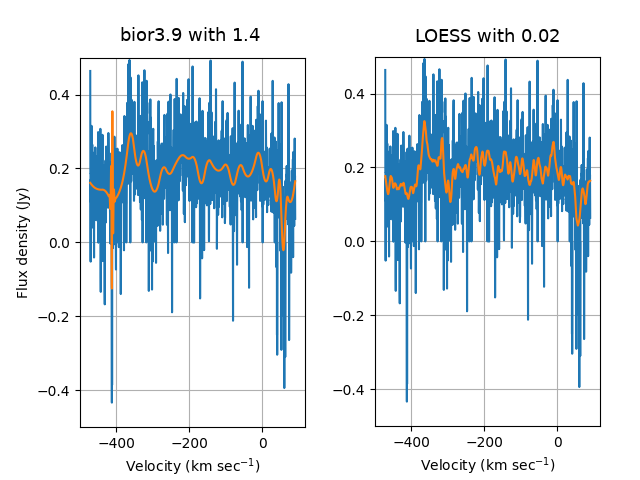
\includegraphics[width=\textwidth]{images/created/method-compare.png}
\caption{Panstarrs C/2017 T2 datu kreisās cirkulārās polarizācijas metožu salīzinājums}
\label{fig:loess}
\end{figure}


\section{ACU žurnalēšanas faili}

Bakalaura darba ietvaros, tika izveidotas vairākas kļūdu kontroles sistēmas, viena no tām - ACU žurnalēšanas failu pārbaudes. ACU jeb Antenna Control Unit ir sistēma, kura atrodas uz Fieldsystem aparatūras \cite{fieldsystem}, kas nodrošina radioteleskopa pozicionēšanu pret novērojuma objektu un informāciju par vēlamo un faktisko teleskopa pozīciju (elevācijas un azimuta vērtības) apraksta žurnalēšanas failos jeb ACU log failos. Šāda veida dokumentēšana nodrošina iespēju zināt precīzu antenu stāvokli konkrētos laikos, līdz ar to, lai pārbaudītu datu integritāti, ACU log failu informācija tika salīdzināta ar novērojumu log failiem.




\begin{figure}[h!]
\centering
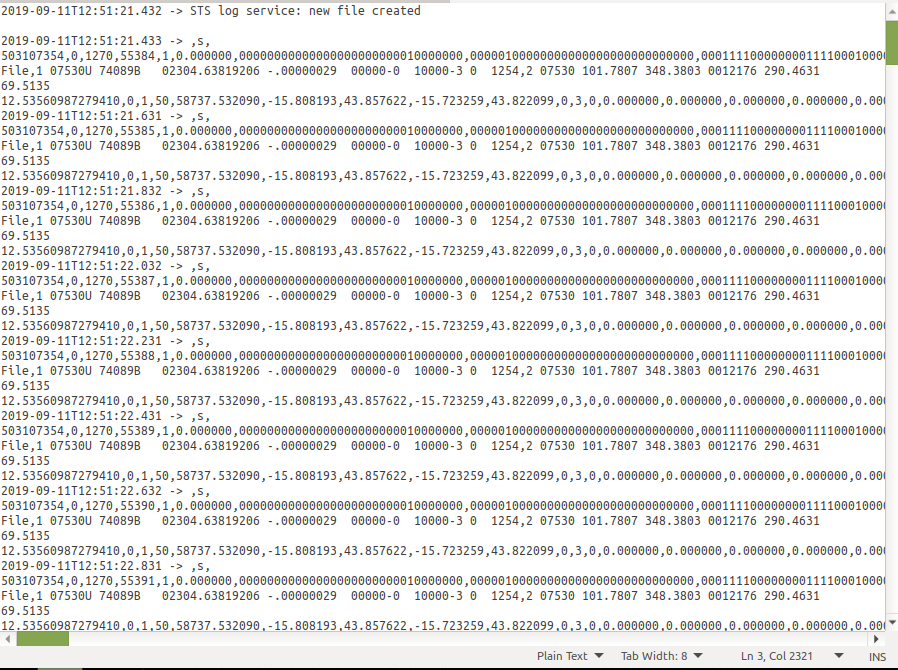
\includegraphics[width=\textwidth]{images/created/acu-img.png}
\caption{ACU sistēmas žurnalēšanas faila piemērs}
\label{fig:acu-example}
\end{figure}

Plašais informācijas daudzums, kurš tiek ierakstīts ACU žurnalēšanas failos arī apgrūtina vieglu informācijas nolasīšanu. Žurnalēšanas faila katra rinda sākās ar ierakstīšanas laiku, kuram seko informācija par ierakstu. Informācija ierakstīta \textit{CSV} stilā, taču informācijai ir ap 200 kolonnām. Ne visas kolonnu vērtības ir vienā formātā, kas vēl vairāk apgrūtina datu nolasīšanu. Vienā žurnalēšanas failā pēc noklusējuma ierakstītas ap 10 000 rindām, kur katrā rindā ir vidēji 2300 simboliem, atkarībā no rindas tipa. Attēlā \ref{fig:acu-example} atspoguļots ACU žurnalēšanas faila sākums no 2019.gada 11. septembra ierakstīšanas sesijām.

Salīdzināšanas sākumā tiek nolasītas visas laika vērtības no novērojuma log faila, kā arī atbilstošās azimuta un elevācijas vērtības šajā laikā. Ņemot vērā, ka ACU logu intervāls starp ierakstiem ir mazāks par 200 milisekundēm, bet novērojumu log failos ierakstu intervāls ir ap 20 sekundēm, identiskus laikus nevar atrast, novērojumu log failu neprecizitātes dēļ. Šī iemesla dēļ tiek izmantots viens no ACU log ierakstiem konkrētā sekundē.  


No ACU logiem tiek nolasīta tekošā pozīcija saskaņā ar enkoderi un uzdotā pozīcija. Nolasītās vērtības tiek salīdzinātas ar novērojumu log failu azimuta un elevācijas vērtībām un tiek izvadīti grafiki salīdzināšanai, kā arī tiek aprēķinātas atšķirības starp vērtībām, izvadot attiecīgus grafikus. Visām šīm vērtībām vajadzētu būt aptuveni vienādām, līdz ar to, ja ir instances kurās vērtības atšķiras, novērojumu skanos ir bojājumi. Grafiki palīdz atrast kļūdas un dod iespēju informēt inženierus par laikiem, kuros anomālijas ir atrastas, lai novērstu problēmas nākotnē.

Grafika piemērs attēlots \ref{fig:acu-example-plot} attēlā, kur aprēķināts OH māzera g126p715 0p822 žurnalēšanas failā ierakstīto elevācijas un azimuta vērtību salīdzinājums ar ACU žurnalēšanas failā ierakstītajām. Rezultāts attēlots, kā sekunžu atšķirība starp abu žurnalēšanas failu  elevācijas vērtībām, konkrētajos laikos. Kā \textit{el\_deltaPlst} un \textit{az\_deltaPlst} tiek attēlots elevācijas un azimuta tekošā pozīcija saskaņā ar enkoderi, bet ar \textit{az\_deltaPsoll} un \textit{el\_deltaPsoll} - uzdotā pozīcija.


\begin{figure}[H]
\centering
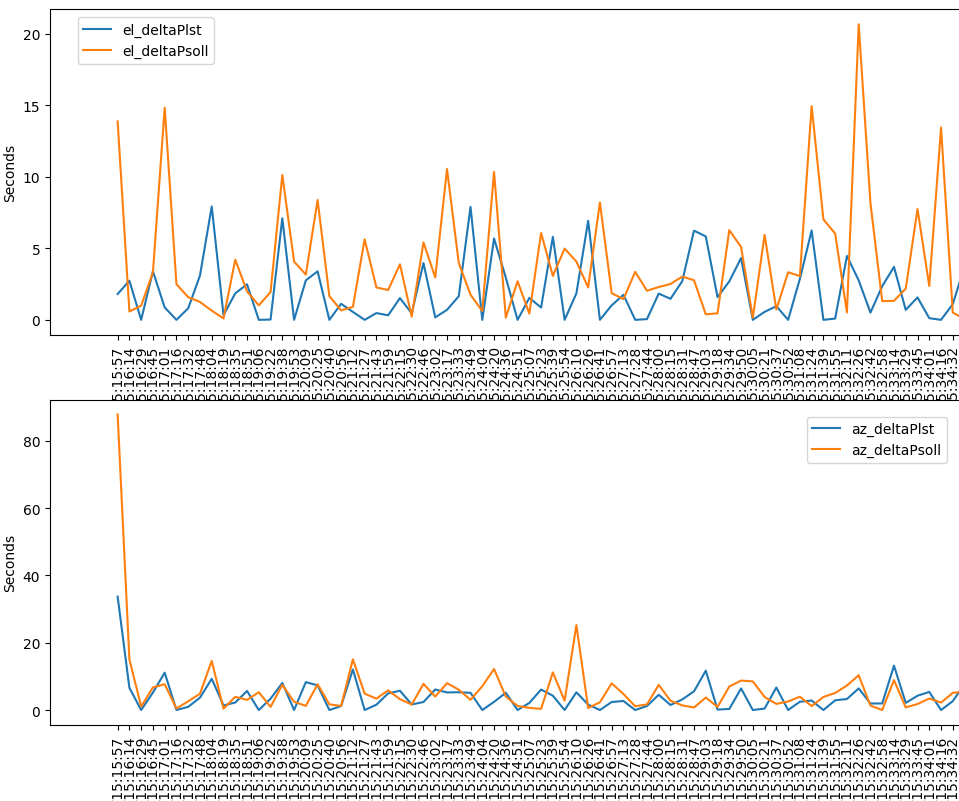
\includegraphics[width=\textwidth]{images/created/ACU-example.png}
\caption{ACU žurnalēšanas faila salīdzinājuma rezultāts}
\label{fig:acu-example-plot}
\end{figure}
%un citi apskatītie
%\subsection{Kalibrācijas integrācija ACOR sistēmā}
%Aprakstīt nedaudz kas tā ir un kas tika izdarīts prakses laikā sakarā ar šo. Aprakstīt kāpēc ir problēmas ar to risinājumu un kā varētu risināt. Ja sanāks laika tad arī risinājumu.

\section{Nākotnes plāni un datu apstrādes tālākie soļi}




Vāju radioastronomisku signālu apstrāde ir sarežģīts process, līdz ar to ir dažādas pieejas katrai problēmai. To efektivitāti iespējams pārbaudīt tikai ar realizāciju, taču visas metodes nebija iespējams apskatīt Bakalaura darba ietvaros, līdz ar to, nodaļā aprakstīti potenciālie uzlabojumi un apstrādes tālākie soļi.

%KLT
Potenciāls uzlabojums apstrādes rezultātos ir iespējams jau datu nolasīšanas brīdī, kur Furjē transformācijas procesu var aizvietot ar Karhunen—Loève Transform \cite{KLT}. Izmantojot minēto apstrādes metodi, tehniski ir iespējams detektēt ļoti vājus signālus attiecībā pret troksni, jo metode izmanto matricu ar nejauši ģenerētiem skaitļiem un veic kompleksus lineārās algebras aprēķinus, lai iegūtu vislabākos koeficientus, kurus izmanto, lai iegūtu spektra frekvenču amplitūdu vērtības. Lai gan vēl nav izpētīts metodes pielietojuma iespējamība radioastronomiskajiem datiem, iespējams, ka, izmantojot minēto metodi, vāju objektu detektēšana būtu efektīvāka.

%Stokes parametri
Lai nodrošinātu datu integritāti un iegūtu papildus informāciju par novērojamo objektu, tika apskatīti arī Stoka \cite{stokes-theory} parametri - vērtību kopa, kas apraksta polarizācijas radiācijas stāvokli. Balstoties uz rakstu par Nançay radioastronomijas observatorijas iegūtajiem rezultātiem 2007.-2009. gada intervālā \cite{nancay}, kurā tika aprakstīta informācija par laika periodā novērotajām maiņzvaigznēm, bija iespējams salīdzināt šos rezultātus ar Bakalaura darba laikā apskatītā objekta rezultātiem. Bakalaura darba ietvaros tika izpētīts \textit{The Measurement of Polarization in Radio Astronomy} \cite{stokes} raksts, lai iegūtu formulas cirkulārās polarizācijas Stokes parametru aprēķinam, taču iegūtos rezultātus nevarēja uzskatīt par pārliecinošiem, līdz ar to tie netiek aprakstīti Bakalaura darba ietvaros.
%\begin{equation}
%I= \langle E_R^2 \rangle + \langle E_L^2 \rangle \tag{2.2.5.1}\label{eq:2.2.5.1}
%\end{equation}
%\begin{equation}
%Q = 2 \langle Re(E_R E_L^*) \rangle = 2 \langle E_R E_L \cos{\delta_{RL}} \rangle \tag{2.2.5.3}\label{eq:2.2.5.3}
%\end{equation}
%\begin{equation}
%U = 2 \langle Im(E_R E_L^*) \rangle = 2 \langle E_R E_L \sin{\delta_{RL}} \rangle \tag{2.2.5.4}\label{eq:2.2.5.4}
%\end{equation}
%\begin{equation}
%V= \langle E_R^2 \rangle - \langle E_L^2 \rangle \tag{2.2.5.5}\label{eq:2.2.5.5} 
%\end{equation}

%\textbf{paskaidrojums un kur/kāpēc tiek izmantots}
%kur: 
%\begin{tabbing}
%\phantom{\hspace{10mm}}\= \kill
%$I$\>                   =$I$\\
%$Q$\>                   = $Q$\\
%$U$\>                   = $U$\\
%$V$\>                   = $V$\\
%$E_R^2$\>               = $E_R^2$\\
%$E_L^2$\>               = $E_L^2$\\
%$\delta_{RL}$\>         = $\delta_{RL}$\\

%\end{tabbing}
%Rakstā tika apskatītas kopā 70 zvaigznes, taču bakalaura darba ietvaros, tika apskatīta tikai informācija par RLMI maiņzvaigni, jo minētais objekts tika novērots, kā komētu kalibrators. 

Stoka parametri sniedz informāciju arī par objekta magnētiskā lauka stāvokli, līdz ar to, papildus izmantojot iegūtos datus kopā ar optiskiem novērojumiem, iespējams veidot OH māzeru spilgtuma modeļus, kā arī veikt objekta monitoringu. Lai gan Bakalaura darbā sadarbība nav realizēta, nākotnē ir potenciāls veidot minēto sadarbību ar kādu optisko novērojumu observatoriju, piemēram, Baldones observatoriju.

Komētu novērojumiem arī ir potenciāls izmantot \textit{Very-Long-Baseline Interferometry} metodes, kur signāls no viena astronomiska objekta tiek novērots ar vairākiem radioteleskopiem vienlaicīgi. Vairāku neatkarīgu staciju novērojumu veikšana vienlaicīgi samazina iespēju veikt inženiertehniskās kļūdas, kā arī sniedz daudz vairāk datu. Lai gan VSRC ir iesaistīts VLBI novērojumos, novērojumu veikšana ir process, kas prasa daudzu staciju sadarbību, kā arī jaunu sistēmu ieviešanu, līdz ar to metodikas ieviešana prasītu ilgu laiku, taču varētu novest pie daudz labākiem rezultātiem.


\chapter{DATU ANALĪZE UN IEGŪTIE REZULTĀTI}




%\section{Novērojuma viekšana?}

\section{Novērojuma apstrāde} \label{data-process}
Novērojuma apstrādes procesu var sadalīt vairākos soļos, katrā solī iegūstot rezultātu. Nodaļā, kā piemērs, tiks apskatīts komētas ATLAS Y4/2019 novērojumu datu rezultāti no 15. marta novērojumu sesijas.
Komētas novērojumi tika plānoti, balstoties uz \ref{planning} nodaļā aprakstītajiem plānošanas soļiem, bet iegūtie novērojuma dati tika apstrādāti balstoties uz 1. nodaļā aprakstītās metodikas. 

\begin{wraptable}{l}{0.5\textwidth}
        \caption{Nodaļā aprakstītā novērojuma informācija}
    \centering
        \begin{tabular}{|l|l|}
        \hline
        Identifikators & atlas\_r\_f1666\_ir\_1 \\ \hline
        Sākuma laiks   & 2020-03-15T04:18:08    \\ \hline
        Beigu laiks    & 2020-03-15T06:34:16    \\ \hline
        Skanu daudzums & 120                    \\ \hline
        FFT garums     & 4096                   \\ \hline
        Joslas platums & 32 MHz                 \\ \hline
        Kanāla platums & 1.526 KHz              \\ \hline
        \end{tabular}
        \label{tab:example-atlas}
\end{wraptable}

Konkrētais novērojums ir izvēlēts kā piemērs, jo ir iespējams attēlot visus 1. nodaļā aprakstītos datu apstrādes soļus. Novērojumam ir pieejami gan jēldati, gan dat formāta faili, kā arī dažos skanos ir detektējamas anomālijas. Novērojuma aktuālā informācija aprakstīta tabulā \ref{tab:example-atlas}.





%\begin{table}[h!]
%\centering
%\begin{tabular}{|l|l|}
%\hline
%Identifikators & atlas\_r\_f1666\_ir\_1 \\ \hline
%Sākuma laiks   & 2020-03-15T04:18:08    \\ \hline
%Beigu laiks    & 2020-03-15T06:34:16    \\ \hline
%Skanu daudzums & 120                    \\ \hline
%FFT garums     & 4096                   \\ \hline
%Joslas platums & 32 MHz                 \\ \hline
%Kanāla platums & 1.526 KHz              \\ \hline
%\end{tabular}
%\caption{Nodaļā aprakstītā novērojuma informācija}
%\label{tab:example-atlas}
%\end{table}

Pirmais iegūtais grafiku tips datu apstrādes procesā ir amplitūdu grafiks, kas ir ticis iegūts, balstoties uz \ref{read-data} nodaļā aprakstītās datu nolasīšanas algoritma. Nolasot visus datus, rezultāti tiek attēloti informatīviem mērķiem un minētās novērojumu sesijas gadījumā tiek iegūti divi grafiki, katrs savam datu tipam (skatīt attiecīgi attēlos \ref{fig:raw-data-atlas}, \ref{fig:dat-data-atlas}). Papildus, rezultātus var izmantot, lai identificētu anomālijas jau pirmajā novērojumu apstrādes fāzē. 

\begin{figure}[H]
\centering
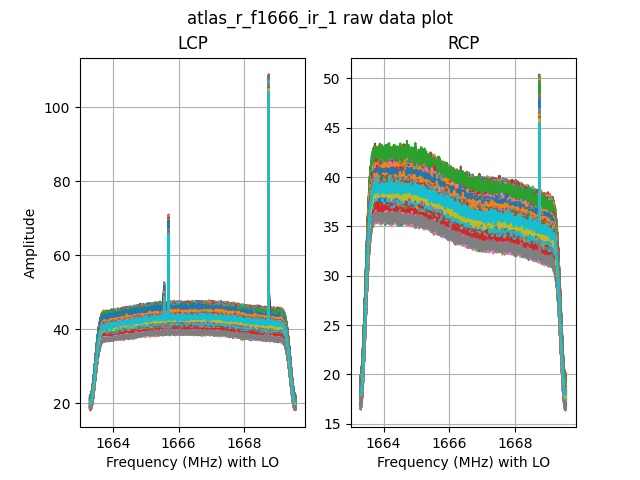
\includegraphics[width=\textwidth]{images/created/atlas-r-f1666-ir-1-raw.png}
\caption{Jēldatu nolasīšanā iegūtais rezultāts}
\label{fig:raw-data-atlas}
\end{figure}

Grafikos \ref{fig:raw-data-atlas}, \ref{fig:dat-data-atlas} attēlotas abas cirkulārās polarizācijas, kā arī visu skanu rezultāti pēc datu nolasīšanas. Rezultātu attēlošanā uz y ass tiek norādīta amplitūda, bet uz x ass - frekvence. Rezultātu iegūšanas brīdī, aprēķini tiek veikti neizmantojot lokālo oscilatoru, taču šiem rezultātiem lokālā oscilatora vērtība tiek pieskaitīta, lai ērtāk orientētos frekvenču joslā. Lai gan novērojumu sesijā vienlaicīgi tiek iegūti abi datu formāti, teleskopu tehnisku grūtību dēļ, iegūtie rezultāti labajā cirkulārajā polarizācijā ir atšķirīgi. Individuālie grafiki apzīmē iegūto rezultātu katrā skanā, līdz ar to katrā polarizācijā ir iegūti 120 spektri.



\begin{figure}[H]
\centering
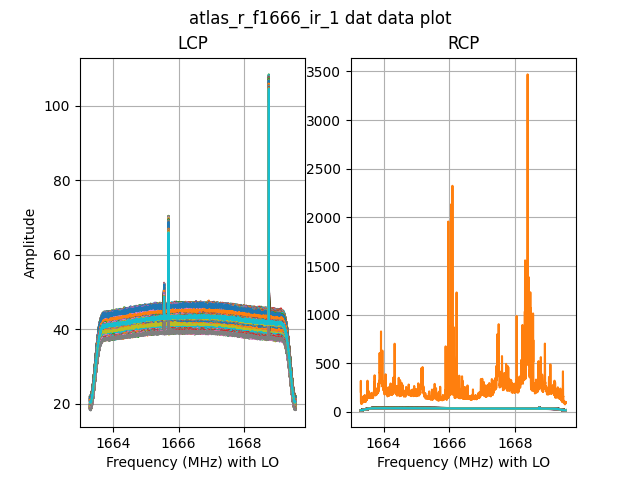
\includegraphics[width=\textwidth]{images/created/atlas-r-f1666-ir-1-dat.png}
\caption{Dat formāta datu nolasīšanā iegūtais rezultāts}
\label{fig:dat-data-atlas}
\end{figure}


Apstrādājot dat failus, iegūtas amplitūdas vērtības norāda, ka novērojuma laikā ir bijušas tehniskas problēmas, jo kreisajā cirkulārajā polarizācijā tiek iegūtas daudz augstākas vērtības noteiktos skanos, salīdzinot ar citiem skaniem. Minētās amplitūdas svārstības netika novērotas jēldatu apstrādes rezultātā, kur iegūtais spektrs nav bojāts, taču tas nenozīmē, ka šiem datiem nav nekādu problēmu. Izmantojot Furjē transformāciju, var iegūt amplitūdu pīķus frekvencēs, kurās avots staro. Pēc spektrālo līniju apraksta \cite{spectral-lines}, OH spektrālajām līnijām ir konkrētas frekvences, kurās OH māzeri staro, līdz ar to, ideālā gadījumā, pīķi būtu novietoti 1665.402 MHz un 1667.359 MHz vērtībās. Aprakstītajā novērojumu sesijas gadījumā ir novērots arī kāds parazītisks signāls, kurš staro citās, bet tuvās frekvenču vērtībās, spēcīgāk par meklēto OH māzeri, kurās pīķis parādās un ietekmē rezultātus.


Lai tālāk analizētu iegūtos datus, ir nepieciešams apskatīt novērojuma sistēmas temperatūras vērtībās. Balstoties uz formulām \ref{eq:1.2.2} un \ref{eq:1.2.3}, kuras aprakstītas \ref{calibration} nodaļā, tiek iegūts \ref{fig:tsys-atlas-raw} attēla grafiks. Bakalaura darba nodaļas ietvaros ir attēlots tikai jēldatu iegūtais rezultāts, jo dat failu rezultāts ir ļoti līdzīgs. Grafikā attēlotas sistēmas temperatūra Kelvinos katrā skana izpildē, kur \textit{LCP ref} un \textit{LCP sig} - kreisās cirkulārās polarizācijas references un objekta sistēmas temperatūras spektri, bet \textit{RCP ref} un \textit{RCP sig} - labās cirkulārās polarizācijas references un objekta sistēmas temperatūras spektri.



%tsys plot
\begin{figure}[H]
\centering
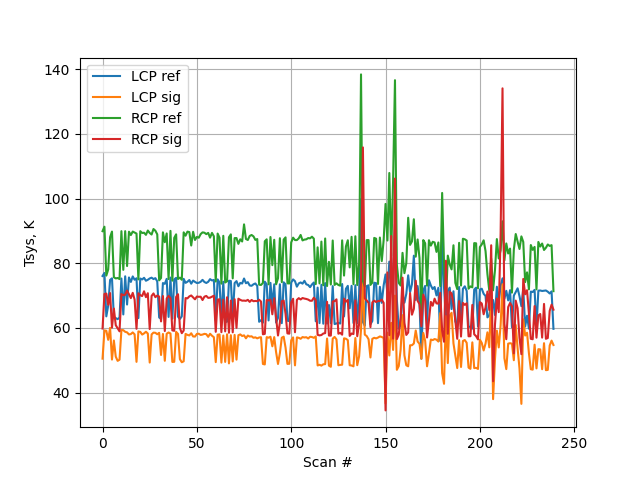
\includegraphics[width=\textwidth]{images/created/tsys-raw-atlas-1.png}
\caption{Jēldatu formāta novērojumā aprēķinātā sistēmas temperatūra}
\label{fig:tsys-atlas-raw}
\end{figure}

Attēlojot sistēmas temperatūras vērtības grafiski, viegli ieraudzīt pēkšņas sistēmas temperatūras izmaiņas. Skani, kuros sistēmas temperatūra pārsniedz normu, spēcīgi negatīvi ietekmēs rezultējošo plūsmas blīvuma spektru, kurš tiek iegūts nākamajā datu apstrādes solī. Pēc \ref{anomalies} nodaļā aprakstītās metodikas, iespējams detektēt minētās izmaiņas algoritmiski. Sākotnēji bojātie skani netika ņemti vērā jēldatu apstrādē, tāpēc bija iespējams apstrādāt mazāku daudzumu datus. Līdz ar to, pareģojot bojāto sistēmas temperatūras vērtību, ir iespējams joprojām izmantot ierakstītos datus.

Izmantojot veivletu transformāciju, var iegūt spektra formu, kura vērtības iespējams izmantot bojātu sistēmas temperatūru gadījumos. Nodaļā aprakstītais rezultāts iegūts izmantojot \textit{rbio1.5} veivletu ar slieksni 3, kas arī ir noklusējuma konfigurācijā. Nodaļā aprakstītā piemēra gadījumā bojātie dati ir detektēti skanos 137, 138, 150, 152, 153, 154, 155, 169, 179, 180, 181, 206, 207, 211, 212, 222. Neizmantojot aprakstīto metodi, bet saglabājot datu integritāti, būtu nepieciešams neapstrādāt 12 skanus jeb 10\% no visiem novērojuma skaniem. Pēc anomāliju detektēšanas un vērtību aizvietošanas, tiek iegūts grafiks \ref{fig:tsys-atlas-modified}, kur papildus grafika \ref{fig:tsys-atlas-raw} sistēmas temperatūras spektriem attēlots arī veivletu transformācijā iegūtie spektri katram sistēmas temperatūras grafikam. Visas iepriekš detektētās skanu sistēmas temperatūras vērtības ir aizvietotas ar vievletu transformācijas rezultējošo vērtību.


\begin{figure}[H]

\centering
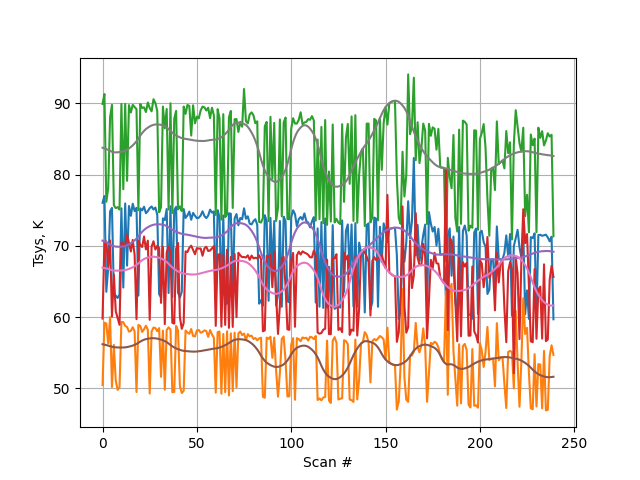
\includegraphics[width=\textwidth]{images/created/atlas-r-f1666-ir-1-tsys-edited.png}
\caption{Jēldatu aprēķinātā sistēmas temperatūra pēc anomāliju identificēšanas}
\label{fig:tsys-atlas-modified}
\end{figure}

Kad iegūtas derīgas sistēmas temperatūras vērtības, ir iespējams kalibrēt \ref{fig:raw-data-atlas} un \ref{fig:dat-data-atlas} grafikos iegūtos rezultātus pēc \ref{calibration} nodaļā aprakstītās metodikas. Kalibrācijas procesā iegūtais rezultāts attēlots \ref{fig:atlas-1-flux} grafikā, kur attēlots abu polarizāciju spektrālās plūsmas blīvums atkarībā no frekvences, izmantojot novērojuma jēldatus. Iegūtais rezultāts no dat tipa datiem ir ļoti līdzīgs, līdz ar to atskaitē nav apskatīts. Salīdzinot attēlos \ref{fig:raw-data-atlas} un \ref{fig:dat-data-atlas} iegūto frekvenču joslu, rezultējošā frekvenču josla ir mazāka, jo interesējošais spektrs ir izgriezts no kopējā. Ar raustītām sarkanām līnijām ir iezīmētas OH māzeru spektrālās līnijas. Ideālā scenārijā, iezīmētājās frekvencēs iespējams iegūt pīķi, 3 reizes izteiktāku par pārējo troksni, bet viena novērojuma rezultātos diemžēl nav iespējams iegūt tik precīzas vērtības apskatītajam objektam.

\begin{figure}[H]
\centering
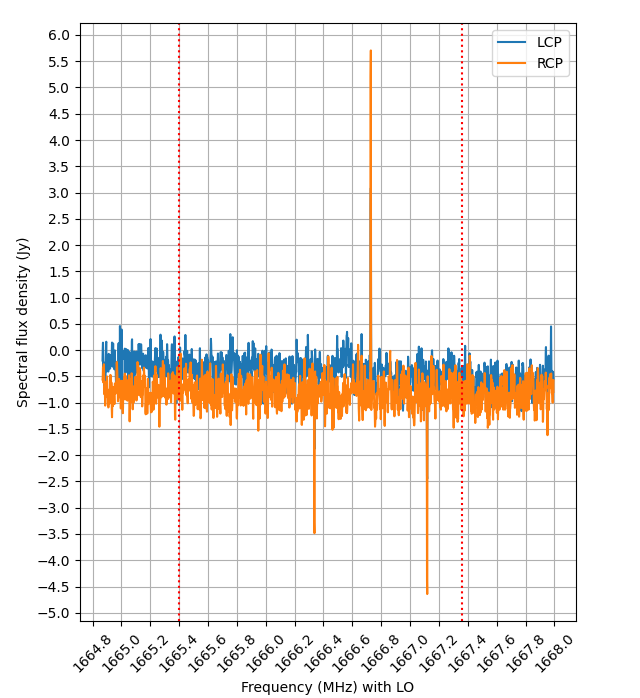
\includegraphics[width=\textwidth]{images/created/atlas-r-1-flux.png}
\caption{Spektrālās plūsmas blīvums atlas-r-f1666-ir-1 datiem.}
\label{fig:atlas-1-flux}
\end{figure}



Izmantojot iepriekš zināmo informāciju, iespējams aprēķināt trokšņa līmeni novērojumā pēc formulas


\begin{equation}
dS = \frac{SFED}{\sqrt{RBW \cdot t}} \tag{2.3.1}\label{eq:2.3.1} 
\end{equation}
kur: 
\begin{tabbing}
\phantom{\hspace{15mm}}\= \kill
$SEFD$\> = Teleskopa jūtība \\
$t$\>   = Novērojuma integrācijas laiks \\
$dS$\>   = Mērījuma troksnis \\
$RBW$\> = Kanāla platums\\

\end{tabbing}

Pēc iekšējā pētījuma rezultātiem \cite{telescope-sefd}, pieņemot, ka teleskopa jūtība ir 700 Jy, kā arī pieņemot, pēc 3 sigmu likuma, ka, lai objektu detektētu, minimālajam objekta plūsmas jaudai jābūt vismaz 3 reizes spēcīgākam par mērījuma troksni, šajā novērojumu iterācijā iegūst aprēķinu:



\begin{equation}
Sf = 3 \cdot dS = 3 \cdot \frac{700 (Jy)}{ \sqrt{1526 (Hz) \cdot 7200 (s) } }\approx 3 \cdot 0.211 (Jy) \approx 0.634 (Jy) \tag{2.3.2}\label{eq:2.3.2} 
\end{equation}
kur: 
\begin{tabbing}
\phantom{\hspace{15mm}}\= \kill
$Sf$\> = Avota spilgtums \\
$dS$\>   = Mērījuma troksnis pēc formulas \ref{eq:2.3.1}\\

\end{tabbing}




\section{Iegūto rezultātu izvērtējums} \label{result-eval}
%Salīdzināšana ar citu zinātnisko avotu rezultātiem, pārbaudes utt.




 %Aprakstīt rezultātus no ATLAS
Balstoties uz to, ka viena novērojuma rezultātā, ar patreizējām tehnoloģijām nevar detektēt signālu, pēc \ref{doppler} nodaļā aprakstītās metodikas iespējams apvienot vairākus novērojumu rezultātus. 

Apskatot iepriekšējā nodaļā novēroto objektu ATLAS Y4/2019 ilgākā laika periodā pēc teorijas iespējams mazināt kopējo trokšņa līmeni novērojumā. Ņemot vērā, ka objekta sadalīšanās veido rezultātu nestabilitāti, ar pielieto metodiku nav iespējams detektēt signālu. Lai iegūtu vairāk informācijas par objektu, ir nepieciešams apskatīt iegūtos datus noteiktos intervālos, kas Bakalaura darba ietvaros nav apskatīts. Lai iegūtu loģisko turpinājumu iepriekšējā nodaļā aprakstītajiem rezultātiem, tiek apskatīts 133 stundu laikā iegūto datu apkopojums jeb 37 dažādu novērojumu rezultāts, atspoguļots \ref{fig:atlas-individ} attēlā, kur ar gradienta palīdzību vecākie dati attēloti, izmantojot gaiši zilu krāsu, bet jaunākie - apzīmēti ar tumši zilu. Pats jaunākais novērojums atzīmēts atsevišķi ar violetu krāsu.
Bakalaura darba atskaitē tiek apskatīta tikai kreisās polarizācijas, 1667 MHz daļas dati, taču iegūtais rezultāts ir pielīdzināms arī pārējām novēroto datu daļām.
\begin{figure}[H]
\centering
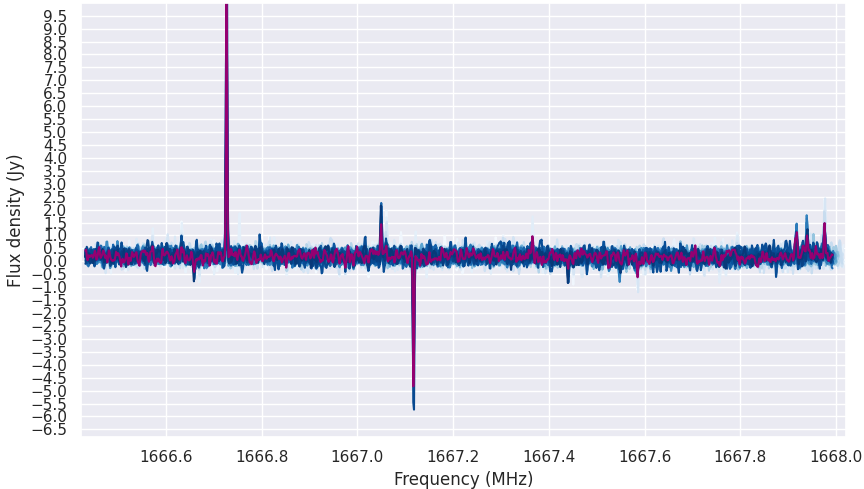
\includegraphics[width=\textwidth]{images/created/atlas-individ.png}
\caption{Visu individuālo novērojumu rezultāts ATLAS Y4/2019 komētas kreisajai cirkulārai polarizācijai.}
\label{fig:atlas-individ}
\end{figure}


Izmantojot attēlā \ref{fig:atlas-individ} iegūtos rezultātus, nav iespējams detektēt signālu nevienā no individuālajiem novērojumiem, līdz ar to, apvienojot visus novērojumus, iegūst \ref{fig:atlas-combined} attēlu, kur reprezentēts interesējošais apgabals kreisās cirkulārās polarizācijas 1667 MHz datu apgabalā, kā arī ar sarkanu līniju iezīmēta OH māzeru starošanas frekvence. Lai gan zemās pīķa maksimālā vērtības dēļ, datu apstrādes rezultāts nevar tikt uzskatīts kā neapstrīdams, ir iespējams, ka tiek detektēts signāls, taču Bakalaura darba ietvaros padziļināti apstrādes rezultāti netiek apskatīti. 

\begin{figure}[H]

\centering
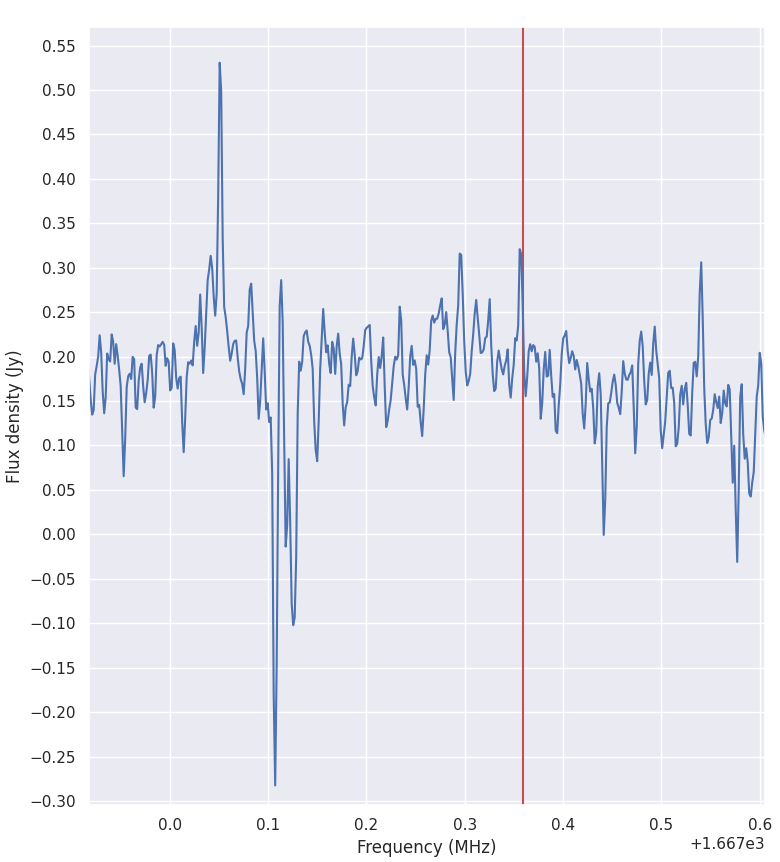
\includegraphics[width=\textwidth]{images/created/1667-atlas-found.png}
\caption{Plūsmas blīvuma atkarība no objekta frekvences ATLAS Y4/2019 kreisās cirkulārās polarizācijas datiem.}
\label{fig:atlas-combined}
\end{figure}




Lai gan komētu novērošanā vēl ir daudz darba, Bakalaura darba ietvaros ir veikts liels progress citu vāju objektu novērošanā. Atsaucoties uz \ref{wavelets} nodaļā aprakstītajiem RLMi rezultātiem attēlā \ref{fig:rlmi-boxed}, izmantojot izveidoto metodiku ir iegūti daudz pārliecinošāki rezultāti. Rezultātus tieši nedrīkst salīdzināt, jo ir daudz ietekmējoši faktori, it īpaši novērojuma ilgums un joslas platuma izmaiņas, taču iegūtie rezultāti liecina, ka objektu var detektēt novērojumu datos ar augstu ticības līmeni.

RLMi maiņzvaigznes patreizējā novērošanas iespējamība attēlota \ref{fig:rlmi-doppler} attēlā, kur attēloti dati no 92 stundu novērojumiem. Lai attēlotu stohastiskā trokšņa samazināšanu, tiek izmantoti grafiki gradienta veidā, kur gaiši zilie spektri atbilst mazāk stundu apvienotajiem novērojumiem, bet tumši zilās atbilst vairāk stundu apvienotajiem novērojumiem. Galējais novērojumu rezultāts iekrāsots violetā krāsā.

\begin{figure}[H]

\centering
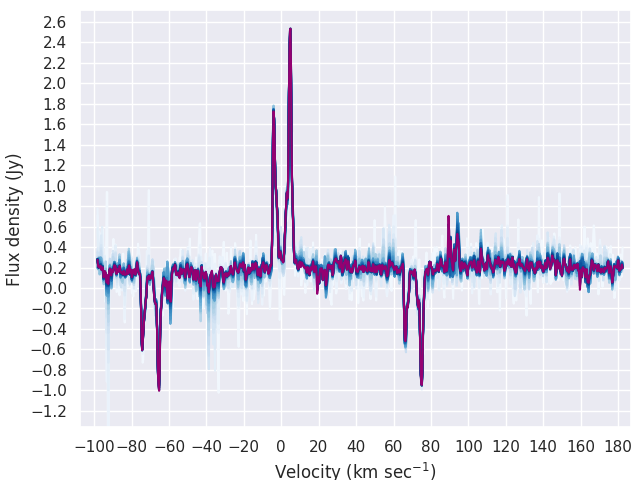
\includegraphics[width=\textwidth]{images/created/rlmi-doppler.png}
\caption{Plūsmas blīvuma atkarība no objekta ātruma maiņzvaigznes RLMi kreisās cirkulārās polarizācijas datiem.}
\label{fig:rlmi-doppler}
\end{figure}
Izmantojot \ref{doppler} nodaļā aprakstīto metodiku, spektra frekvenču josla tiek pārrēķināta uz objekta ātruma vērtībām. Pēc datu apstrādes, rezultējošajā spektrā, ir iegūti pīķi -4 km/s un 5 km/s vērtībās, kas arī pēc aprēķiniem ir novērotā OH māzera pārvietošanās ātruma vērtības ar augstu trokšņa pret signāla attiecību.


\section{Bakalaura darba izstrādes laikā novērotie kosmiskie objekti} \label{objects}


Bakalaura darba ietvaros tika novēroti vairāki radioastronomiski objekti, kurus var iedalīt kategorijās - maiņzvaigznes, komētas un zvaigžņu veidošanās apgabali.

Novērojot vājus objektus, lai nodrošinātu datu integritāti, nepieciešams kāds spēcīgāks avots, kuru vieglāk detektēt. Bakalaura darba novērojumu ietvaros tika izmantota maiņzvaigzne R Leonis Minoris (turpmāk RLMi). Balsoties uz rakstu no Nancay radioastronomijas observatorijas Francijā, \cite{nancay} tika salīdzinātas iegūtās vērtības ar Irbenē iegūtajām un tika iegūts līdzīgs rezultāts. Kopš tā brīža, RLMi tika novērots visās novērojumu sesijās, kur tiek novērota komēta Saules sistēmā.

Iegūstot rezultātus uz salīdzinoši spēcīgā avota RLMi, bija iespējams novērot arī komētas Saules sistēmā, kuras izstaro vāju OH māzera starojumu. Pirmā novērotā komēta, kura tika apskatīta Bakalaura darba ietvaros ir Panstarrs C/2017 T2 (turpmāk Panstarrs). Ņemot vērā, ka objekta orbīta nodrošina ilgstošu redzamību, komēta ir novērota visilgāko laiku. Lai gan komēta ir salīdzinoši vāja spilgtuma - vidēji ap 12 magnitūdām pēc NASA HORIZONS datiem novērojumu veikšanas laikā, ilgais novērošanas laiks dod iespēju efektīvāk pārbaudīt ar vairāku novērojumu apvienošanu saistītu metodiku.

Asteroid Terrestrial-impact Last Alert System jeb ATLAS 2019 gada 28. decembrī atklāja jaunu komētu - ATLAS C/2019 Y4 (turpmāk Atlas). Gada beigās atklātajai komētai tika aprēķinātas augstas spilgtuma vērtības, kas sniedza iespēju daudziem zinātniekiem to novērot. Komētu klasificē kā Kreutz sungrazer tipa komētu, kas nozīmē, ka komētas perifērijas ir ļoti tuvu Saulei. Lai gan tas pozitīvi ietekmē komētas spilgtumu, tas palielina iespējamību komētām sadalīties, kas arī notika ar Atlas komētu ap 2020. gada 1. aprīli \cite{atlas-frag}.   Komētas orbīta liecina, ka Atlas komēta ir bijusi daļa no Lielās komētas C/1844 Y1 \cite{atlas-article}, bet atdalījusies aptuveni piecu tūkstošu gadu atpakaļ. Komētai sadaloties, stipri palielinās komētas spilgtums, taču sadalīšanās brīdī komētai veidojas vairākas daļas, kur nereti katrai daļai ir savs kodols. Kodolā esošo OH molekulu daudzums vairs nav tik daudz, līdz ar to starojuma jauda samazinās, kas noved pie samazinātām komētas novērošanas iespējām.

Lai gan Atlas komētas sadalīšanās nozīmēja komētas novērošanas beigas, Saules sistēmā parādījās jauna spoža komēta - SWAN C/2020. Pirmo reizi atklāta, izmantojot Solar and Heliospheric Observatory jeb $SOHO$. Swan komēta tika atklāta, jo tā izvadīja kosmosā ļoti lielu daudzumu $H_2O$ \cite{swan-disc}. Komēta Bakalaura darba nodevuma laikā joprojām tiek novērota un darbs pie datu apstrādes turpinās.

\begin{table}[h!]
\centering
\caption{Bakalaura darba izstrādes laikā ilgstoši novērotās komētas}.
\begin{tabular}{|c|l|l|l|l|l|}
\hline
\textbf{Objekta nosaukums} & \textbf{Atlas C/2019 Y4} & \textbf{Panstarrs C/2017} & \textbf{Swan C/2020 F8}  \\ \hline
\textbf{Tuvākā distance līdz Zemei} & 0.781 AU & 1.5202 AU  &  0.557 AU  \\ \hline
\textbf{Tuvākā distance līdz Saulei} & 0.253 AU & 	1.615 AU &  0.432 AU  \\ \hline
\textbf{Spilgtums perihēlija punktā}           & Sadalījusies & 8.6  &  7.6   \\ \hline
\textbf{Objekta novērojuma ilgums}       & 133h 16m 47s & 149h 21m 54s &  110h 09m 57s \\ \hline
\textbf{Novērojumu sākuma datums}       & 2020-Mar-14 & 2020-Jan-26 &  2020-May-05 \\ \hline
\textbf{Pēdējais novērojumu datums}       & 2020-Apr-11 & 2020-May-04 &  2020-May-20 \\ \hline

%\multicolumn{1}{|l|}{}                   &  &  &  &  &  &  &  &  &  \\ \hline
\end{tabular}

\label{tab:main-objects}
\end{table}

% Objekta nosaukums & Tuvākā distance līdz Zemei & Maksimālais spilgtums & Objekta novērojuma ilgums\\

Neskaitot primārās komētas, kuras aprakstītas \ref{tab:main-objects} tabulā\footnote{Distances un spilgtuma dati no astro.vanbuitenen.nl}, tika arī novērotas sekojošās komētas: C/2018 N2 (ASASSN), C/2019 B1 (Africano), 284P/McNaught, taču minētie objekti bija pārāk vāji novērošanas laikā, vai bija tehniskas problēmas, kuras liedza veikt ilgstošus novērojumus.


%\begin{table}[h!]
%\centering
%\begin{tabular}{|c|l|l|l|l|l|}
%\hline
%\multicolumn{4}{|c|}{Mazāk novērotās komētas}                            \\ \hline
%\textbf{Objekta nosaukums} & \textbf{Mcnaught} & \textbf{Africano} & %\textbf{Assasn}  \\ \hline
%\textbf{Tuvākā distance līdz Zemei (KM)} &  &  &    \\ \hline
%\textbf{Tuvākā distance līdz Saulei (KM)} &  &  &    \\ \hline
%\textbf{Maksimālais spilgtums}           & ???  & ???  &  ???   \\ %\hline
%\textbf{Objekta novērojuma ilgums}       & ??? & ??? &  ??? \\ \hline
%\multicolumn{1}{|l|}{}                   &  &  &  &  &  &  &  &  &  \\ \hline
%\end{tabular}
%\caption{Bakalaura darbā novērotās komētas Saules sistēmā}
%\label{tab:min-objects}
%\end{table}


Bakalaura darba izstrādes laikā, tika novērotas ne tikai komētas Saules sistēmā, bet arī radioastronomiski māzeri, kas staro spēcīgāk par komētām. Viens no tiem bija metanola māzeris Cepheus A zvaigžņu veidošanās apgabalā. Balstoties uz to, ka objekts tika novērots jau iepriekš, bija zināms, ka tā pīķis sasniedz 180 Jy vērtību, līdz ar to, objekts tika izmantots, lai testētu jēldatu apstrādes algoritmu uz cita veida datiem. Spēcīgu māzeru novērojumos parasti nav nepieciešams izmantot jēldatu formātu, jo dat faili sniedz pietiekami labu precizitāti, līdz ar to metodika, kā apstrādāt māzeru jēldatus nebija izveidota, taču šajā datu līmenī, starpība starp objektiem ir ļoti maza, līdz ar to, var izmantot to pašu apstrādes procesu. Māzeru apstrāde sniedza iespēju efektīvāk identificēt kļūdas, jo spektram bija iepriekš zināma forma, ar ko varēja salīdzināt iegūtos datus, kas nav iespējams komētu novērojumiem.

Papildus minētajiem novērojumiem, Bakalaura darba izstrādes laikā tika novērots vēl viens vājš OH māzeris - g126p715 0p822, kurš tika izmantots līdzīgiem nolūkiem, bet rezultātiem būtu jābūt līdzīgākiem komētu OH māzeru novērojumu rezultātiem. Māzera novērošanas laiks bija ļoti īss, kā arī novērojumu laikā bija tehniskas problēmas, kuras neļāva iegūt vēlamos rezultātus. Izmantojot datus no minētā māzera, kā arī dienu iepriekš novērotās C/2019 B1 (Africano) komētas, varēja identificēt, ka teleskopā ir problēmas, jo bija izteikts troksnis konkrētās frekvenču vērtībās.




%Spēcīgs avots novērojumu testēšanai:

%\textbf{RLMi}

%Komētas:

%\textbf{PANSTARRS (C/2017 T2)}

%\textbf{ATLAS (C/2019 Y4)}

%Mazāk novērotās:

%\textbf{Mcnaught}

%\textbf{Africano}

%\textbf{Assasn}

%Galaktiskie māzeri:

%\textbf{cepa}

%\textbf{g126p715 0p822}

%Nākotne:

%\textbf{C/2020 F8 (SWAN), C/2020 F3 (NEOWISE), C/2019 U6, 2P/Encke}


%\textbf{aprakstīt visus objektus, kā arī kapēc tie tiek izmantoti}






\chapter{ALGORITMA IZVĒRTĒJUMS} \label{algorithm-eval}


\section{Datu apstrādes tehniskā informācija}


Ņemot vērā, ka VSRC pārvaldībā ir nonācis jauns skaitļošanas klasteris, bija iespēja pielietot algoritmu uz jaunas paaudzes skaitļošanas klastera. Līdz ar to, bija iespējams veikt veiktspējas testus uz lielāka resursu daudzuma, salīdzinot ar parasti pieejamo, un apskatīt algoritma veiktspēju atkarībā no dažādu parametru konfigurācijas. Lai vairāk kontrolētu datu apstrādes vidi, tika izmantotas virtuālās mašīnas uz VSRC skaitļošanas klastera.


\begin{table}[h!]
\centering
\caption{Veiktspējas testos izmantoto individuālo virtuālo mašīnu apraksts}
\begin{tabular}{|l|l|}
        \hline
        Procesora ligzdas & 2 \\ \hline
        Procesora kodoli ligzdā & 48 \\ \hline
        BIOS   & SeaBIOS    \\ \hline
        Procesora tips    & kvm64   \\ \hline
        Atmiņa & 325.96 GB                    \\ \hline
        \end{tabular}
        
        \label{tab:vm-info}
\end{table}


Balstoties uz to, ka klastera mezgli izmanto \textit{Proxmox} operētājsistēmu, kas piedāvā iebūvētas virtuālo mašīnu veidošanas tehnoloģijas, tika izveidotas trīs virtuālās mašīnas ar tabulā \ref{tab:vm-info} aprakstītajiem parametriem. Virtuālajām mašīnām tika ielādēta \textit{Ubuntu 19.10 Live Server} versija, kā arī papildus noklusējuma bibliotēkām, tika instalētas \textit{openmpi} pakotnes, kā arī nepieciešamās bibliotēkas datu apstrādes skripta realizācijai. Skaitļošanas mezgli savā starpā saslēgti izmantojot 10GB/s optiskos kabeļus. Dati atrodas ārējā datu serverī, kas pieslēgts katrai virtuālajai mašīnai. Lai veiktu veiktspējas testus, tiek izmantoti dati no 2.2. nodaļā aprakstītā novērojuma.


\section{Veiktspējas testi}

Veicot veiktspējas testus, ir jāņem vērā daudz faktori, līdz ar to ideālu veiktspējas testu izpilde nav viegla. Faktori, kā ielasīšanas ātrums ir noteicoši konkrētā veida datu apstrādes algoritmos, līdz ar to ir limitācijas, cik ļoti ir iespējams uzlabot algoritma veiktspēju. Izveidojot pilnībā simulētu vidi, zūd algoritma veiktspējas uzticamība, salīdzinot ar veiktspēju reālajā pasaulē.

Veiktspējas testi ir veikti, izmantojot \textit{Linux} pakotni \textit{hyperfine}\cite{hyperfine}. Pakotne veidota, lai ērti nodrošinātu veiktspējas testu veikšanu, izmantojot nepieciešamos parametrus. Lai iegūtu salīdzinoši kontrolētus rezultātus, visiem nodaļā aprakstītajiem veiktspējas testiem tiek izmantotas 5 \textit{warmup} iterācijas, kā arī 30 rezultātu mērītās iterācijas.

Lai vieglāk atsauktos uz algoritma versijām, kuras tiek apskatītas, nodaļas ietvaros \textit{pirmā} versija MPI algoritmam apzīmē 1.5 nodaļā aprakstīto pirmo algoritmu, kurš attēlots pielikumā \ref{appendix:old-version}, bet \textit{pēdējā} versija apzīmē 1.5 nodaļā aprakstīto otro algoritmu, kurš attēlots pielikumā \ref{appendix:new-version}.

Lai attēlotu veiktspējas uzlabojumus no \textit{pirmās} MPI algoritma algoritma iterācijas un \textit{pēdējās}, ņemot vērā vienādu kodolu skaitu (9), rezultāti tiek atspoguļoti kastveida diagrammā \ref{fig:old-v-new} attēlā, kur ar violeto krāsu tiek attēloti rezultāti no \textit{pirmās} algoritma iterācijas, bet ar zaļo tiek attēlots \textit{pēdējās} algoritma iterācijas veiktspēja. Tehniski jēldatus \textit{pēdējā} versijā apstrādā par vienu procesu mazāk nekā \textit{pirmajā} versijā, taču tiek ņemts vērā, ka abi algoritmi katrs aizņem deviņus procesus kopā. 



Ņemot vērā, ka datos ir izlecošās vērtības, biežākais izpildes laiks tiek mērīts, izmantojot mediānas vērtību. Pēc veiktspējas testu rezultātiem, \textit{pirmās} versijas algoritms visbiežāk izpildīsies aptuveni 3193.2148 sekundēs, kamēr \textit{pēdējā} algoritma versija izpildīsies aptuveni 2535.8932 sekundēs. 


Jāņem arī vērā, ka \textit{pirmajā} algoritmā nav integrētas anomāliju pārbaudes, kuras aprakstītas nodaļā \ref{anomalies}, kā arī papildus datu izveide, līdz ar to, ja \textit{pēdējā} algoritma darba skaits tiktu pielīdzināts \textit{pirmajam}, tā veiktspēja būtu vēl sliktāka. Lai gan \textit{pirmā} algoritma darbībai, pēc teorijas, vajadzētu būt ātrākai, \textit{pēdējā} algoritma ietvaros tiek izmantoti dažādi augstas veiktspējas risinājumi problēmām, it īpaši ciklu vektorizācija, kas izteikti minimizē darbību ilgumu.

\begin{figure}[H]
\centering
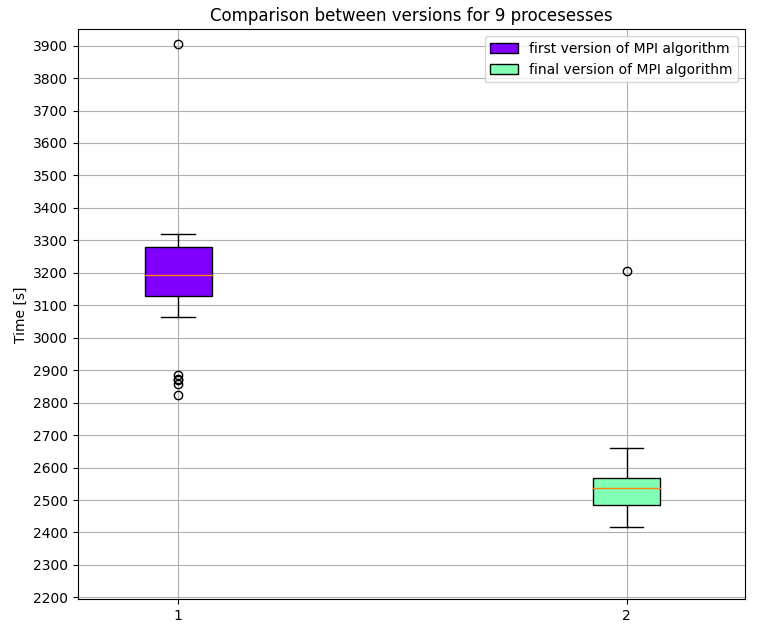
\includegraphics[width=\textwidth]{images/created/old-v-new.png}
\caption{Pirmā datu apstrādes algoritma veiktspējas salīdzinājums ar pēdējās versijas veiktspējas salīdzinājumu.}
\label{fig:old-v-new}
\end{figure}


\textit{Pēdējais} algoritms ir tieši atkarīgs no procesu skaita un failu daudzuma. Ideālā gadījumā, datu apstrādē algoritmam būtu iespējams  apstrādāt katru failu savā procesā, taču, lai to realizētu 4 stundu gariem novērojumiem, būtu nepieciešams paredzēt 1920 kodolus datu apstrādei, kas patreizējā situācijā ir reti iespējams. Pēc teorijas, palielinot kodolu daudzumu, izpildes laiks samazināsies.

Lai attēlotu \textit{pēdējās} versijas algoritmu, tiek apskatīts veiktspējas rezultāts atkarībā no pieejamiem resursiem. Attēlā \ref{fig:all-bench} tiek atspoguļoti rezultāti izmantojot 9, 64, 192 un 234 procesus. Iegūtie rezultāti no 9 un 64 procesu datiem ir apstrādāti vienas virtuālās mašīnas ietvarā, bet 192 un 234 procesu rezultāti, izmantojot visu virtuālo mašīnu kopējos skaitļošanas resursus. 






\begin{figure}[H]
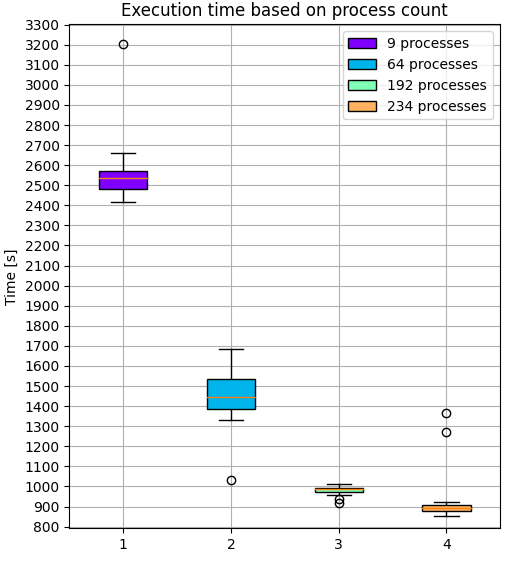
\includegraphics[width=\textwidth]{images/created/all-bench-rez.png}

\caption{\textit{Pēdējā} algoritma veiktspēja atkarībā no procesu skaita}
\centering
\label{fig:all-bench}
\end{figure}

Lai gan Bakalaura darba ietvaros nav apskatīts pats sākotnējais algoritms, kurš realizēts bez MPI iekļaušanas, tipiska novērojuma apstrādāšanai bija nepieciešamas aptuveni 5 stundas.



\section{Algoritma potenciālie uzlabojumi}

Algoritma veiktspējas uzlabošanas lielākais šķērslis ir algoritma procesu pārvaldības procesa optimizācija, jo apskatot kodolu noslodzi, var noteikt, ka algoritma izpildes sākuma posmā visi izsauktie kodoli izpildās uz 100\% noslodzi, taču, kad pirmie faili nolasīti, uz pārvaldības procesu vienlaicīgi tiek sūtītas vairākas ziņas no apstrādes procesiem par nolases pabeigšanu. Tas nozīmē, ka ir nepieciešams apstrādāt visus ienākošos procesus, piešķirot atbrīvojušajiem procesiem jaunu failu apstrādei, kā arī klausīties jeb nodrošināt pārējo procesu statusu monitoringu. Visas aprakstītās darbības prasa skaitļošanas laiku, līdz ar to nevar efektīvi pārvaldīt visus pieejamos procesus. Problēmas risinājums būtu ieviest vairāk-pārvaldības procesus, lai gan minētais uzlabojums varētu ļoti sarežģīt algoritma loģiku. Lai gan patreizējā \textit{numpy} vektorizācija ir daudz efektīvāka, salīdzinot ar ciklu pieeju, ir ieteicams izmantot iebūvētās \textit{MPI} funkcijas, kuras nodrošinātu efektīvāku procesu komunikāciju.



Veicot datu apstrādes algoritmu optimizāciju, ir iespējams izmantot divas pieejas, kur katrai ir savi izmantošanas plusi un mīnusi. Pirmā pieeja, kuru savā ziņā arī izmanto \textit{pirmais} MPI algoritms, ir statiski norādīt instrukcijas katram procesam un katru reizi algoritma izpildē izmantot statisku procesu daudzumu. Minētais risinājums ļoti uzlabo kopējo veiktspēju, jo tiek samazināts komunikāciju daudzums starp procesiem, kā arī realizācija ir daudz vienkāršāka, izmantojot nemainīgas instrukcijas, tādējādi veidot pilnībā kontrolētu vidi. Bet kopumā aprakstītais risinājums padara algoritmu nemērogojamu. Izmantojot \textit{pirmo MPI} algoritmu, nav iegūti augstākas veiktspējas rezultāti par jaunākās versijas rezultātiem, jo starp iterācijām tika apgūtas dažādas augstas veiktspējas labās prakses, kas krasi uzlaboja veiktspēju.

Ņemot vērā, ka pieejamais skaitļošanas resursu daudzums var mainīties, nav garantēts konkrēts kodolu skaits algoritma izpildei, bija nepieciešams izmantot otro pieeju - zaudēt statiskās instrukcijas katram procesam un dinamiski atļaut procesu pārvaldību. Minētā pieeja vienmēr samazinās kopējo veiktspēju, jo procesiem savā starpā jāsazinās un jāinformē par procesa stāvokli, bet visbiežāk, izveidojot algoritmu pēc minētās metodes, ir iespējams iegūt labāku veiktspēju kopumā, vienkārša iemesla dēļ - programrisinājumam ir pieejami vairāk skaitļošanas resursi.

Ņemot vērā, ka Bakalaura darba ietvaros koda optimizācija un kopējā veiktspēja ir svarīgs faktors, jāņem vērā, ka patreizējā sistēma pilnībā ir realizēta Python programmēšanas valodā. Tā tika izvēlēta atvieglotai algoritma realizācijai, plašo bibliotēku atbalsta un vienkāršotās sintakses dēļ, bet valodai dēļ tās izpildes laika interpretatora ir izteiktākas tehniskās limitācijas. Izmantojot \textit{numpy} bibliotēku var efektīvi vektorizēt darbības, kā ciklu izpildi un matricu manipulāciju, bet pilnībā optimizēts kods visticamāk būs lēnāks par pilnībā optimizētu kodu zemāka līmeņa valodā, kā C, pateicoties faktam, ka kods tiek interpretēts izpildes laikā. Diemžēl nav iespējams izvērtēt algoritma pārrakstīšanas guvumu neieguldot daudzas stundas pārrakstīšanā, līdz ar to konkrētus rezultātus konkrētajā jautājumā nevar iegūt.

%\input{src/nakotnes-plani}
%Nodaļu un apakšnodaļu skaits netiek reglamentēts, tas izriet no darba apjoma un satura.
%Problēmas teorētiskais izklāsts varētu aizņemt aptuveni 50\% no analītiskās daļas kopapjoma. Tomēr tas nedrīkst būt literatūras konspekts, bet gan attiecīgā temata izvērtējums.














%Nodaļai nevar būt tikai viena apakšnodaļa. Analītiskās daļas  uzdevums ir sistematizētā veidā sniegt pētāmās problēmas īsu teorētisku pamatojumu, autora pētījuma rezultātus, kas formulēti priekšlikumu veidā. Visās analītiskās daļas nodaļās (izņemot teorētisko pamatojumu) jābūt ilustratīvajam materiālam un aprēķiniem: konkrētiem plāna aprēķiniem, analītiskām tabulām, diagrammām u.tml. Problēmas teorētiskais izklāsts varētu aizņemt aptuveni 50\% no analītiskās daļas kopapjoma. Tomēr tas nedrīkst būt literatūras konspekts, bet gan attiecīgā temata izvērtējums.

%\section{Datu apstrādes metodikas implementācija}















%Te ievietosim attēlu. Attēlam ir jāatrodas iepriekš definētajā mapē \verb+./PNG+. Šajā piemērā tiek izmantots attēls \verb+./PNG/Answer_to_Life.png+

%Atbilde uz mūs interesējošo jautājumu ir parādīta \ref{fig:answer}~attēlā. Attēls rasts tīmeklī

%\begin{figure}[ht] \centering
% Norādam ievietojamo failu - paplašinājumu png var nerakstīt
%\includegraphics[width=0.95\textwidth]{Answer-to-Life}
%% pievienojam nosaukumu ar avotu un atsauci - label , ko var izmantot tekstā ar ref
%\caption{Pati galvenā atbilde\cite{ans-picture}}  \label{fig:answer}
%\end{figure}

%\subsection{Par izmantoto literatūru un avotiem}

%Izmantotās literatūras un avotu saraksts aptver literatūras avotus, kas izmantoti darba izstrādāšanā

%Izmantotās literatūras un avotu saraksta veidošanas mērķis ir pateikties šo darbu autoriem par viņu ieguldījumu, parādīt darba lasītājam, no kurienes autors ir ņēmis attiecīgo informāciju un ļaut lasītājam pārbaudīt izmantoto informāciju no pirmavotiem.

%Nedrīkst pieļaut plaģiātismu (cita autora darba uzdošanu par savu). Studentu, kuru darbs tiek atzīts par plaģiātu tiek atstādināti no pārbaudījuma un eksmatrikulē. Atkārtota darba aizstāvēšana tiek atļauta ne ātrāk kā pēc gada, un darbs ir jāraksta par jaunu tematu.

%Bieži plaģiātismu izraisa nekorekta citēšana vai atsauču neievietošana darba tekstā. Ja darbā izmanto precīzas citu autoru frāzes vai teksta fragmentus, tad nepietiek tikai ar atsauci, šādos gadījumos jāizmanto citāts, kas jāliek pēdiņās. Atsauce ir obligāta arī tad, ka students pārfrāzē cita autora domas.


%% Nenumurēta nodaļa, kas uzrādās satura rādītājā
\chapter*{SECINĀJUMI UN PRIEKŠLIKUMI}
\addcontentsline{toc}{chapter}{SECINĀJUMI UN PRIEKŠLIKUMI}

Darba gaitā ir sasniegts izvirzītais mērķis - veikt vāju radioastronomisko objektu datu apstrādi, to kalibrāciju,  trokšņa filtrēšanu, analizēt un apkopot iegūtos rezultātus. Veicot darbu, autors secināja:

\begin{enumerate}

    \item Lai realizētu datu apstrādes algoritmu, bija nepieciešams apgūt radioastronomisko novērojumu teorētiskos pamatus, kā arī Irbenes novērojuma stacijā lietoto infrastruktūru, ieskaitot datu formātus un ierakstīto informāciju.
    \item Algoritmu izveide, balstoties uz zinātniskajiem rakstiem, nereti ir izaicinošs process, jo informācija  rakstā var tikt interpretēta dažādos veidos. Minētais faktors, kopā ar nepilnīgām zināšanām radioteleskopa darbībā, noveda pie grūtībām pilnībā izprast kalibrācijas procesa darbību, kas sarežģīja uzlabojumu ieviešanu.
    \item Veicot datu apstrādi, nepieciešams pārliecināties par iepriekšējiem datu apstrādes procesiem, jo nepietiekama informācija noved pie kļūdainas tālākas apstrādes. Ņemot vērā, ka nav pieejamas specifiski aprakstītas dokumentācijas par iepriekšējiem datu apstrādes procesiem, tas noveda pie apjukuma situācijās, kur, piemēram, tika apskatīta Doplera kompensācija, kas daļēji jau bija realizēta datu ierakstīšanas brīdī.
    \item Apskatot vairākas apstrādes metodes, dažkārt ir vērts ieguldīt ilgāku laiku metodes izpratnei, jo metode var sniegt pielietojumu dažādās jomās. Tas pierādījās apskatot veivletu transformāciju, kuru bija iespējams pielietot ne tikai stohastiskā trokšņa samazināšanā, bet arī sistēmas temperatūru bojāto vērtību pareģošanā.
    \item Apstrādājot datus, ir nepieciešams izvērtēt potenciālās paralelizācijas iespējas, kā arī izpētīt vairākus iespējamos variantus paralelizācijas realizācijai. Izmantojot MPI paralelizāciju, vairāku stundu ilgā datu apstrāde tika aizstāta tikai ar maksimāli pus stundu garu datu apstrādes procesu.
    \item Veicot algoritmu paralelizāciju, ir nepieciešams ņemt vērā algoritmisko nestabilitāti. Vienmēr jāpārliecinās, ka izsauktais process pilda instrukcijas, kas procesam ierādītas. Pat ja algoritms ir paralelizēts, tam ir iespējams veikt dažādus vienkāršus uzlabojumus, kā piemēram ciklu vektorizēšanu, kas noved pie daudz labākas veiktspējas. Bakalaura darbā tas izpaudās algoritma iterāciju salīdzināšanā, kur, lai gan pirmās iterācijas algoritms veica mazāk darba, izpildījās lēnāk par pēdējās iterācijas algoritmu. 
    \item Vāju radioastronomisko objektu datu apstrādes metodes dažkārt sniedz nepārliecinošus rezultātus, līdz ar to ir nepieciešams salīdzināt iegūtos rezultātus ar citu metožu rezultātiem, piemēram, ar rezultātiem no optiskajiem novērojumiem.
    \item Veicot zinātnisku algoritmu izveidi, nepieciešams konsultēties ar jomas ekspertiem rezultātu analizēšanai, kā arī potenciālu uzlabojumu ieteikumiem. Radioastronomisko datu apstrādes rezultāti, bieži ir sarežģīti uzskatāmi, jo ne vienmēr ir skaidrs, kā izskatīsies rezultāts, taču izmantojot metodes no iepriekšējās pieredzes, ir iespējams efektīvāk apstrādāt datus, kā arī gūt pārliecību par iegūtajiem rezultātiem.   
    \item Iegūstot datus no ārējiem avotiem, ir jāpārliecinās par avotu uzticamību, kā arī nepieciešams būt pārliecinātam, ko iegūtie dati reprezentē. Resursi, kā piemēram, NASA HORIZONS satur ļoti daudz informācijas, taču dažkārt datu daudzums izraisa apjukumu. Tiek ierakstītas dažādas ātruma vērtības, atkarībā no citiem objektiem, rezultātā, iegūstot līdzīgas, bet tomēr, nedaudz atšķirīgas vērtības. Apskatot arī datus, kā pareģotā objekta spilgtuma vērtība, bieži dažādos resursos ir atšķirīga, lai gan objekts ir viens. Dati iegūti no dažādām datubāzēm un bieži tiek izmantoti atšķirīgi algoritmi, lai iegūtu pareģotas vērtības, kas izraisa atšķirīgu gala rezultātu.
    %\item Infrastruktūra bieži ir nedokumentēta vai nepilnīgi dokumentēta, kas sarežģī jaunu algoritmu izveidi vai vecu algoritmu uzlabojumus.
    \item Populārās programmēšanas valodās, kā piemēram Python vai C, populārām problēmām bieži ir augstas veiktspējas risinājumi, kurus izmantojot, kopējā algoritma veiktspēja var vairākas reizes uzlaboties.
    \item Vāju radioastronomisku objektu novērošana ir sarežģīts darbs, līdz ar to, ir nepieciešams pārbaudīt vairākas un atšķirīgas signālu apstrādes metodes uz kādiem konkrētiem datiem, lai pārliecinātos par iegūto rezultātu pareizību.
    
    \item Veicot datu apstrādi, ir nepieciešams aprakstīt iegūtos rezultātus dokumentācijā, kas autoram ļauj labāk izprast kopējos rezultātus, kā arī atskaites atļauj citiem pētniekiem labāk izprast algoritmiski realizētos problēmu risinājumus.
    
    

    
\end{enumerate}

Līdz ar to, no iepriekš izdarītajiem secinājumiem, autors sniedz šādus priekšlikums:
\begin{enumerate}
    
    \item  Izstrādātā algoritma procesu komunikācijas realizācija efektīvākā veidā nodrošinātu daudz labāku veiktspēju datu apstrādes algoritma izpildē. To iespējams realizēt, izmantojot statiskas instrukcijas noteiktam procesu daudzumam vai ieviešot papildus pārvaldes procesus.
    \item Algoritma veiktspēju iespējams optimizēt, izmantojot zemāka līmeņa valodu, taču izstrādes process prasītu ilgu laiku, jo liela daļa funkciju realizētas izmantojot \textit{Python} pakotnes.
    \item Bakalaura darba ietvaros realizēto Doplera nobīdes aprēķināšanu Saules sistēmas objektiem būtu nepieciešams izvērtēt, jo iegūtie rezultāti ir nepārliecinoši.
    \item Autors iesaka apskatīt papildus datu apstrādes metodes, piemēram,  Karhunen—Loève Transform metodi Furjē transformācijas vietā, kas, iespējams, sniegtu precīzākus rezultātus, jo metode paredzēta vāju signālu apstrādei, izmantojot nejaušu skaitļu un statistikas elementu aprēķinus. Transformācijas rezultātā, varētu būt iespējams samazināt stohastiskā trokšņa ietekmi, apstrādātajos rezultātos.
    \item Papildus apskatītajiem novērojuma datiem, ir nepieciešams apskatīt objekta Stoka parametrus, kas atļautu iegūt vairāk informāciju par objekta polarizācijas radiācijas stāvokli un objekta magnētiskā lauka stāvokli.

    \item Ņemot vērā faktoru, ka radioteleskops ir ļoti kompleksa sistēmu kopa, novērojumu laikā var rasties inženiertehniskas problēmas. Lai gan biežāko problēmu risinājumi ir ieviesti, ir nepieciešams padziļināti apskatīt problēmu sekas uz iegūtajiem datiem, kā arī veikt attiecīgās pārbaudes.
    \item Komētas ir ieteicams novērot, izmantojot vairākas stacijas, gan optiskajā diapazonā, gan izmantojot citu radioteleskopu staciju datus, veidojot VLBI tipa novērojumos, jo tas sniegtu daudz vairāk datu, kā arī novērstu potenciālās inženiertehniskās problēmas.
\end{enumerate}

%\begin{enumerate}
%\item \textbf{Secinājumi un priekšlikumi} jāraksta tēžu veidā.
%\item Secinājumiem jāatspoguļo svarīgākās atziņas, kas izriet no pētījuma, satur atbildes uz ievadā izvirzīto mērķi un uzdevumiem.
%\item Secinājumos jāpaskaidro veiktā pētījuma tautsaimnieciskā, zinātniskā vai praktiskā nozīme un autora personīgais veikums uzdevuma risināšanā.
%\item Secinājumus nedrīkst pamatot ar datiem un faktiem, kas nav minēti darbā.
%\item Secinājumos nav pieļaujami citāti no citu autoru darbiem, tajos jāatspoguļo tikai darba autora domas, spriedumi, atziņas.
%\item Priekšlikumiem jāizriet no darbā veiktajiem pētījumiem un izdarītajiem secinājumiem, tiem jābūt konkrētiem un pamatotiem.
%\item Priekšlikumos apkopo arī darbā pamatotās rekomendācijas trūkumu novēršanai.
%\item Secinājumi un priekšlikumi jānumurē ar arābu cipariem.
%\end{enumerate}
 %% Ērtāk visu failā secinajumi-un-priesklikumi.tex


\bibliographystyle{unsrt}
\selectlanguage{latvian}
\bibliography{src/links,src/articles,src/books}	%to load the *.bib files ../articles,../books,
\addcontentsline{toc}{chapter}{IZMANTOTĀS LITERATŪRAS UN AVOTU SARAKSTS}



%% Te vajadzētu pielikumus
\appendix
\chapter{ATLAS C/2019 Y4 REDZAMĪBAS GRAFIKS}


Attēlā apskatīts Atlas C/2019 Y4 komētas elevācijas vērtības, atkarībā no laika. Ar sarkanu iekrāsots potenciālo novērojumu laiku intervāls, kas komētai iespējams visu laiku, jo visas vērtības ir virs 15 grādus sliekšņa. Attēls tiek apskatīts, jo attēlo atšķirīgu komētu potenciālo novērojumu iespēju. Komētu novērojumi iespējami daudz vieglāk realizējami nekā \ref{fig:swan-el} attēlā apskatītās SWAN  C/2020 F8 novērojumi. Dati iegūti no NASA HORIZONS sistēmas.


\begin{figure}[H]
\centering
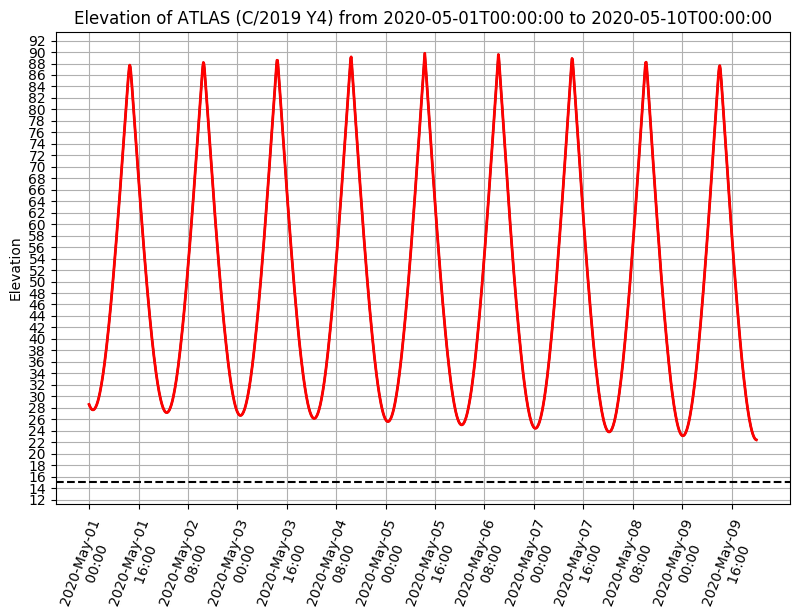
\includegraphics[width=\textwidth]{images/created/atlas-visibility.png}
\label{fig:atlas-visibility}
\end{figure}

%\begin{figure}[htb]
%  \centering
%  \begin{turn}{-90}
%  \begin{minipage}{\textheight}
%  \centering
%    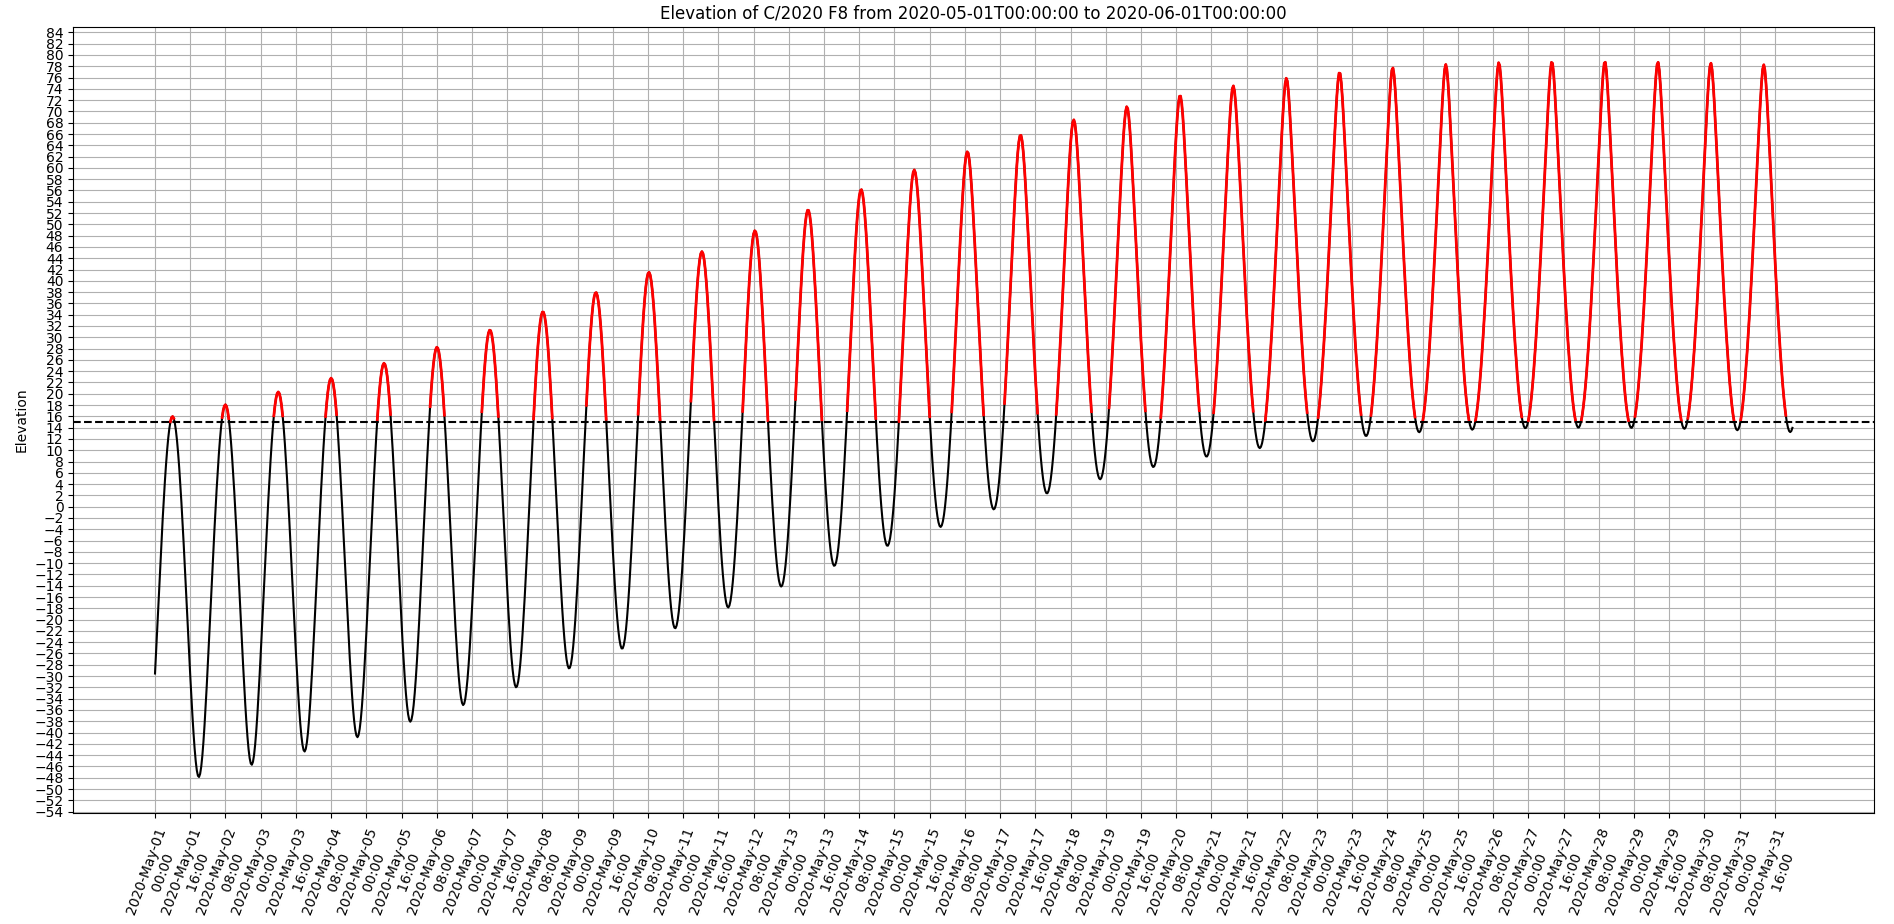
\includegraphics[width=\textwidth]{images/created/swan-bigger.png%}
%  \label{fig:bigger-swan}
%  \end{minipage}
%  \end{turn}
%\end{figure}






\addtocounter{nofappendices}{1}
\label{appendix:tituldati}
%\lstinputlisting[firstline=6, lastline=15]{../codes/calcHomogInfModel.m}
%\lstinputlisting[firstline=18, lastline=25]{README.md}

\chapter{MPI ALGORITMA PIRMĀS VERSIJAS IZPILDES PROCESA ATTĒLOJUMS}

Attēlā tiek apskatīts, kā notiek procesu komunikācija un datu apstrādes plūsma pirmajā MPI algoritma versijā. Procesi sadalīti celiņos, kur katrs celiņš atbilst katram procesam. Pirmais process veic datu kalibrāciju un apkopošanu, kamēr pārējie - jēldatu apstrādi. Process katrā solī tiek attēlots kā aplis, kura iekšienē tiek norādīts, kurš fails no kopējās novērojumu datu kopas tiek apstrādāts. 

Katrā datu apstrādes ciklā, tiek apstrādāti 8 faili, kuru failu nosaukumus process nr. 1 nosūta pārējiem procesiem. Kad dati nolasīti, katrs process nosūta iegūtos rezultātus pirmajam procesam, kurš rezultātus nokalibrē un uzglabā atmiņā. Pēc kalibrācijas, tiek izsūtīta nākamā 8 failu kopa procesiem un process tiek atkārtots, līdz visi faili apstrādāti. Kā N zīmējumā tiek apzīmēts kopējais failu skaits.

Procesa kodu var apskatīt \ref{appendix:codes} pielikuma repozitorijā, kur mapē \textit{scripts} atrodas fails \textit{MPI\_calibr\_v1.py}, kurā ir veikts pilns datu apstrādes process izmantojot pielikumā aprakstīto metodi.

\begin{figure}[h!]
  \centering
  \begin{turn}{-90}
  \begin{minipage}{\textheight}
  \includesvg[width=\textwidth]{images/created/old-algorithm.svg}
  \end{minipage}
  \end{turn}
\end{figure}

\addtocounter{nofappendices}{1}
\label{appendix:old-version}

\chapter{MPI ALGORITMA FINĀLA VERSIJAS IZPILDES PROCESA ATTĒLOJUMS}

Attēlā tiek apskatīts, kā notiek procesu komunikācija un datu apstrādes plūsma pēdējā MPI algoritma versijā. Procesi sadalīti celiņos, kur katrs celiņš atbilst katram procesam. Pirmais process veic datu kalibrāciju un apkopošanu, otrais process realizē procesu pārvaldību, trešais process - dat formāta failu apstrādi, kamēr pārējie - jēldatu apstrādi. Trešais process arī veic jēldatu apstrādi pēc dat formāta datu apstrādes beigšanas. 

Process katrā solī tiek attēlots kā aplis, kura iekšienē tiek norādīts procesa statuss. Ja process ieņem vērtību "1", process ir brīvs un to var izmantot datu apstrādei.

Balstoties uz faktoru, ka katra faila nolasīšanas laiks var nedaudz atšķirties, arī komunikācija starp procesiem var atšķirties. Piemērā pirmie procesi, kuri beidz datu nolasīšanu ir process nr. 8 un nr. 6, bet realitātē nav iespējams pateikt kurš process beigs datu apstrādi pirmais. Nosacījums izpildās arī pārējos soļos. Pārvaldības process izsūta visus failu ceļus datu apstrādes procesiem, bet kad visi faili izsūtīti, pārējiem procesiem aizsūta ziņu par datu apstrādes beigām. Procesi saņemot ziņu, nosūta datu apstrādē iegūtos rezultātos procesam 1, kurš veic tālāku datu apstrādi un beidz darbību.

Procesa kodu var apskatīt \ref{appendix:codes} pielikuma repozitorijā, kur mapē \textit{scripts} atrodas fails \textit{MPI\_calibr\_v2.py}, kurā ir veikts pilns datu apstrādes process izmantojot pielikumā aprakstīto metodi.


\begin{figure}[h!]
  \centering
  \begin{turn}{-90}
  \begin{minipage}{\textheight}
  \includesvg[width=\textwidth]{images/created/new-algorithm.svg}
  \end{minipage}
  \end{turn}
\end{figure}




\addtocounter{nofappendices}{1}
\label{appendix:new-version}
%\lstinputlisting{README.md}


\chapter{BAKALAURA DARBA IETVAROS VEIDOTIE KODI}

Ņemot vērā kodu apjomu, lai iegūtu labāku algoritmu uzskatāmību, kods nav apskatīts Bakalaura darba apraksta ietvaros, bet pieejams publiskā, Bakalaura autora veidotā \textit{github} repozitorijā. Repozitorijā ir divas direktorijas - \textit{scripts} un \textit{docs}, kur kodi apskatāmi \textit{scripts} direktorijā, bet Bakalaura gala apraksta Latex pirmkods, kopā ar darbā izmantotajiem vizuālajiem materiāliem, apskatāms \textit{docs} direktorijā.

Piekļuve repozitorijam iespējama, izmantojot: \\
\url{https://github.com/dot361/Weak-radio-signal-data-processing}, vai pēc pieprasījuma.


\addtocounter{nofappendices}{1}
\label{appendix:codes}

\chapter*{GALVOJUMS}
\addcontentsline{toc}{chapter}{GALVOJUMS}
 Ar šo es, \defAutors, galvoju, bakalaura darbs ir izpildīts patstāvīgi un bez citu palīdzības. No svešiem pirmavotiem ņemtie dati un definējumi ir uzrādīti darbā. Šis darbs tādā vai citādā veidā nav nekad iesniegts nevienai citai pārbaudījumu komisijai un nav nekur publicēts.

\vspace{2cm}
\defGads.gada \rule{1cm}{0.2pt}.\rule{3cm}{0.2pt}
\hspace{100pt} \rule{4cm}{0.2pt}
\vspace{2cm} 


 Es, \defAutors, atļauju Ventspils Augstskolai savu bakalaura darbu bez atlīdzības ievietot un uzglabāt Latvijas Nacionālās bibliotēkas pārvaldītā datortīklā Academia (www.academia.lndb.lv), kurā tie ir pieejami gan bibliotēkas lietotājiem, gan globālajā tīmeklī tādā veidā, ka ikviens tiem var piekļūt individuāli izraudzītā laikā, individuāli izraudzītā vietā.

\hspace{180pt} Piekrītu \hspace{15pt} \rule{5cm}{0.2pt}

\vspace{8pt}

\hspace{180pt} Nepiekrītu \hspace{2pt} \rule{5cm}{0.2pt}

\vspace{2cm}
\defGads.gada \rule{1cm}{0.2pt}.\rule{3cm}{0.2pt}
\vspace{2cm}


\label{LastPage}
%% Vēl jāpievieno atzīmes lapa
%\pagebreak
%% Šai lapai nevajag numerāciju
%\pagestyle{empty}
%\begin{center}
% Bakalaura darbs aizstāvēts Valsts pārbaudījumu komisijas sēdē\\
% \vspace{1em}
%\end{center}
%\defGads.gada \rule{1cm}{0.2pt} . \rule{3cm}{0.2pt}\\\\
%un novērtēts ar atzīmi \rule{4cm}{0.2pt} \\\\\\
%Protokols Nr. \rule{1cm}{0.2pt}\\\\\\
%Valsts pārbaudījumu komisijas \\\\
%priekšsēdētājs \rule{7cm}{0.2pt}.\\
%\hspace*{5cm}\textit{\raisebox{1em}{paraksts}}


\end{document}
